\documentclass[a4paper]{article}

% -------------------------------------------------------------------- %
%                                                                      %
% fichier de préambule                                                 %
%                                                                      %
% Importantion de nombreux packages, plus francisation                 %
%                                                                      %
% -------------------------------------------------------------------- %

% ----------------------------------------------------------------------
% gestion du français, et des accents
\usepackage{cmap}
\usepackage[T1]{fontenc}
\usepackage[english,frenchb]{babel}
\usepackage[utf8]{inputenc}
\usepackage{helvet}
\usepackage{courier}
%\renewcommand{\familydefault}{\sfdefault}
%\pdfcompresslevel=3
%\usepackage{fourier}

\usepackage{datetime} % pour avoir l'heure de compilation avec \currenttime

\usepackage{color}
\usepackage[table]{xcolor}

\usepackage{sectsty}
\allsectionsfont{\bfseries\sffamily\color{black!90}\hspace{-1em}}
\partfont{\sffamily}
\usepackage[font={small,it}]{caption}
\makeatletter
\def\@seccntformat#1{\llap{\csname the#1\endcsname\quad}}
\makeatletter\pdfcompresslevel=9
\def\@seccntformat#1{\llap{\csname the#1\endcsname\quad}}
\makeatother

% ----------------------------------------------------------------------
% bibliography
\usepackage[backend=biber, bibencoding=utf8 , sorting=none,hyperref=true,url=false,backref=true,backrefstyle=three]{biblatex}
\bibliography{input/biblio}

% ----------------------------------------------------------------------
% packages pour les figures
\usepackage{graphicx}
\usepackage{subfig}
\usepackage{tikz}

% change la numéroration des figures
%%%% debut macro %%%%
\makeatletter
\renewcommand{\thefigure}{\ifnum \c@section>\z@ \thesection.\fi
 \@arabic\c@figure}
\@addtoreset{figure}{section}
\makeatother
%%%% fin macro %%%%

% change la numéroration des tableaux
%%%% debut macro %%%%
\makeatletter
\renewcommand{\thetable}{\ifnum \c@section>\z@ \thesection.\fi
 \@arabic\c@table}
\@addtoreset{table}{section}
\makeatother
%%%% fin macro %%%%

% ----------------------------------------------------------------------
% diagramme de Gantt
%\usepackage{model/pgfgantt}

% ----------------------------------------------------------------------
% pour mettre une page en mode paysage
\usepackage{lscape}

% ----------------------------------------------------------------------
% Miscelianous
\usepackage[pdfborder={0 0 0 [3 3]},pdftex,unicode=true]{hyperref}
\usepackage{bookmark}

%\usepackage{tablefootnote}

% ----------------------------------------------------------------------
%packages pour les maths
\usepackage{amsmath}
\usepackage{amssymb}
\usepackage{mathabx} %   \ldbrack et \rdbrack
%\usepackage{amsfonts}
\usepackage{mathrsfs}
\usepackage{wasysym}
\usepackage{textcomp}
%\usepackage{bbm}
\DeclareMathAlphabet{\mathpzc}{OT1}{pzc}{m}{it} % \mathpzc{ABCdef}
\usepackage{eufrak}                             % \mathfrak{ABCdef}

% change la numéroration des équations
\numberwithin{equation}{section}

% ----------------------------------------------------------------------
% pour les unités
%\usepackage[load=physical]{siunitx}
\newcommand{\eV}{\mathrm{eV}}
\newcommand{\s}{\mathrm{s}}
\newcommand{\m}{\mathrm{m}}
\newcommand{\g}{\mathrm{g}}
\newcommand{\V}{\mathrm{V}}
\newcommand{\sample}{\mathrm{s}}
\newcommand{\Hz}{\mathrm{Hz}}
\newcommand{\pc}{\mathrm{pc}}

\newcommand{\nano}{\mathrm{n}}
\newcommand{\micro}{\mathrm{\mu}}
\newcommand{\milli}{\mathrm{m}}
\newcommand{\centi}{\mathrm{c}}
\newcommand{\kilo}{\mathrm{k}}
\newcommand{\mega}{\mathrm{M}}
\newcommand{\giga}{\mathrm{G}}
\newcommand{\tera}{\mathrm{T}}
\newcommand{\exa}{\mathrm{E}}
\newcommand{\zetta}{\mathrm{Z}}


% ----------------------------------------------------------------------
% packages pour les algorithmes
\usepackage[section]{algorithm}
\usepackage[noend]{algpseudocode}

\renewcommand{\algorithmiccomment}[1]{{\hfill$\vartriangleright$\scriptsize\sffamily~ #1}}

% francisation des algorithmes
\floatname{algorithm}{\sffamily Algorithme}

\renewcommand{\algorithmicprocedure} {{\footnotesize \textbf{\textsf{Proc\'edure}} }}
\renewcommand{\algorithmicwhile}     {{\footnotesize \textbf{\textsf{Tant que}}    }}
\renewcommand{\algorithmicdo}        {{\footnotesize \textbf{\textsf{Faire}}       }}
\renewcommand{\algorithmicend}       {{\footnotesize \textbf{\textsf{Fin}}         }}
\renewcommand{\algorithmicif}        {{\footnotesize \textbf{\textsf{Si}}          }}
\renewcommand{\algorithmicelse}      {{\footnotesize \textbf{\textsf{Sinon}}       }}
\renewcommand{\algorithmicthen}      {{\footnotesize \textbf{\textsf{Alors}}       }}
\renewcommand{\algorithmicfor}       {{\footnotesize \textbf{\textsf{Pour}}        }}
\renewcommand{\algorithmicforall}    {{\footnotesize \textbf{\textsf{Pour tout}}   }}
\renewcommand{\algorithmicdo}        {{\footnotesize \textbf{\textsf{Faire}}       }}
\renewcommand{\algorithmicrepeat}    {{\footnotesize \textbf{\textsf{Répéter}}     }}
\renewcommand{\algorithmicuntil}     {{\footnotesize \textbf{\textsf{Jusqu'à}}     }}
\renewcommand{\algorithmicfunction}  {{\footnotesize \textbf{\textsf{Fonction}}    }}
\renewcommand{\algorithmicreturn}    {{\footnotesize \textbf{\textsf{Retourner}}   }}
\let\mylistof\listof
\renewcommand\listof[2]{\mylistof{algorithm}{Liste des algorithmes}}
\makeatletter
\providecommand*{\toclevel@algorithm}{0}
\makeatother
% Lister les algorithmes :
%\listofalgorithms % même principe que toc
\addto\captionsfrench{%
  \renewcommand{\listfigurename}{Liste des figures}%
}
\addto\captionsfrench{\def\figurename{Figure}}
\addto\captionsfrench{\def\tablename{Tableau}}

% ----------------------------------------------------------------------
% tableaux
\definecolor{tablegray}{gray}{0.8}%table

% ----------------------------------------------------------------------
% importantion de code
\definecolor{mygray}{rgb}{0.5,0.5,0.5} % définition du gris (n° ligne)
\usepackage{listings}
\usepackage{listingsutf8}

% couleurs pour listings
\definecolor{lightgray}{rgb}{.9,.9,.9}
\definecolor{darkgray}{rgb}{.4,.4,.4}
\definecolor{purple}{rgb}{0.65, 0.12, 0.82}

% javascript definition
\lstdefinelanguage{Javascript}{
  keywords={typeof, new, true, false, catch, function, return, null, catch, switch, var, if, in, while, do, else, case, break},
  keywordstyle=\color{blue}\bfseries,
  ndkeywords={class, export, boolean, throw, implements, import, this},
  ndkeywordstyle=\color{darkgray}\bfseries,
  identifierstyle=\color{black},
  sensitive=false,
  comment=[l]{//},
  morecomment=[s]{/*}{*/},
  commentstyle=\color{purple}\ttfamily,
  stringstyle=\color{red}\ttfamily,
  morestring=[b]',
  morestring=[b]"
}

% pour la numerotation des codes
\usepackage{chngcntr}
\AtBeginDocument{\counterwithin{lstlisting}{section}}

\renewcommand{\lstlistlistingname}{Liste des extraits de code}
%%options for listings
\DeclareCaptionFont{white}{\color{white}}
\DeclareCaptionFormat{listing}{\colorbox{black!80}{\parbox{\textwidth}{#1#2#3}}}
\captionsetup[lstlisting]{format=listing,labelfont={white,tt},textfont=white}
\definecolor{Rred}{rgb}{0.6,0,0} % for strings
\definecolor{Rgreen}{rgb}{0.25,0.5,0.35} % comments
\definecolor{Rpurple}{rgb}{0.5,0,0.35} % keywords
\definecolor{Rdocblue}{rgb}{0.25,0.35,0.75} % Rdoc
\lstset{
    float,
    columns=fullflexible,
    numbers=left,
    tabsize=2,
    breaklines=true,
    basicstyle=\small\ttfamily,
    basewidth=0.51em,
    showspaces=false,
    showstringspaces=false,
    stringstyle=\color{Rred},
    commentstyle=\color{Rgreen},
    keywordstyle=\color{Rdocblue}
}
% gestion des accents dans le code
\renewcommand{\lstlistingname}{Code}
\lstset{literate=
    {á}{{\'a}}1 {é}{{\'e}}1 {í}{{\'i}}1 {ó}{{\'o}}1 {ú}{{\'u}}1
    {Á}{{\'A}}1 {É}{{\'E}}1 {Í}{{\'I}}1 {Ó}{{\'O}}1 {Ú}{{\'U}}1
    {à}{{\`a}}1 {è}{{\`e}}1 {ì}{{\`i}}1 {ò}{{\`o}}1 {ù}{{\`u}}1
    {À}{{\`A}}1 {È}{{\'E}}1 {Ì}{{\`I}}1 {Ò}{{\`O}}1 {Ù}{{\`U}}1
    {ä}{{\"a}}1 {ë}{{\"e}}1 {ï}{{\"i}}1 {ö}{{\"o}}1 {ü}{{\"u}}1
    {Ä}{{\"A}}1 {Ë}{{\"E}}1 {Ï}{{\"I}}1 {Ö}{{\"O}}1 {Ü}{{\"U}}1
    {â}{{\^a}}1 {ê}{{\^e}}1 {î}{{\^i}}1 {ô}{{\^o}}1 {û}{{\^u}}1
    {Â}{{\^A}}1 {Ê}{{\^E}}1 {Î}{{\^I}}1 {Ô}{{\^O}}1 {Û}{{\^U}}1
    {œ}{{\oe}}1 {Œ}{{\OE}}1 {æ}{{\ae}}1 {Æ}{{\AE}}1 {ß}{{\ss}}1
    {ç}{{\c c}}1 {Ç}{{\c C}}1 {ø}{{\o}}1 {å}{{\r a}}1 {Å}{{\r A}}1
    {€}{{\EUR}}1 {£}{{\pounds}}1
}

% ----------------------------------------------------------------------
% trucs en vracs
\usepackage[         %
    top    = 2.75cm, %
    bottom = 3.50cm, %
    left   = 3.00cm, %
    right  = 2.50cm]{geometry}   % marges
\usepackage{makeidx}             % make index (finalement je ne l'utilise pas)
\makeindex                       % génération de l'index, besoin d'une compilation séparée

\usepackage{fancyhdr}            % entête et pied de page (pour les modifier)
\pagestyle{fancy}                % style des pages
\fancyhf{}
\renewcommand{\sectionmark}[1]{\markboth{\thesection{} -- #1}{}}
\fancyhead[L]{\leftmark}
\fancyhead[R]{\thesubsection}
\makeatletter
\fancyfoot[L]{\@author \space --- \schoolShortName{} }
\makeatother 
\fancyfoot[R]{\thepage}
\renewcommand{\footrulewidth}{0.1pt}

\usepackage{setspace}     % gestion des interlignages
\onehalfspacing           % interlignage de 1.5

% ----------------------------------------------------------------------
%Page de titre
\newcommand{\HRule}{\rule{\linewidth}{0.5mm}}
\usepackage{model/titlepage}

% ----------------------------------------------------------------------
% modification du style des parties (pour la classe article)
\makeatletter
\renewcommand\part{%
  \clearpage
  \thispagestyle{empty}%
  \null\vfill
  \secdef\@part\@spart}
\def\@part[#1]#2{%
    \ifnum \c@secnumdepth >-2\relax
      \refstepcounter{part}%
      \addcontentsline{toc}{part}{\thepart\hspace{1em}#1}%
    \else
      \addcontentsline{toc}{part}{#1}%
    \fi
    \markboth{}{}%
    {\centering
     \interlinepenalty \@M
     \vskip 20\p@
     \normalfont
     \ifnum \c@secnumdepth >-2\relax
       \huge\bfseries \partname\nobreakspace\thepart
       \par
       \vskip 20\p@
     \fi
     \Huge \bfseries\sffamily #2\par}%
    \@endpart}
\def\@spart#1{%
    {\centering
     \interlinepenalty \@M
     \vskip 20\p@
     \normalfont
     \Huge \bfseries #1\par}%
    \@endpart}
\def\@endpart{\vfill
              \newpage
              }
\makeatother


\renewcommand*{\thefootnote}{(\arabic{footnote})}
% ----------------------------------------------------------------------
% nouvelles commandes
\newcommand{\fraction}[2]{\raisebox{0.5ex}{#1}\slash\raisebox{-0.5ex}{#2}}
% pour afficher 1/2, ne fonctionne pas dans un environnement mathématique

\newcommand{\ie}{\emph{i.e.}}
\newcommand{\eg}{\emph{e.g.}}

\newcommand{\Cpp}{\emph{C++}}
\newcommand{\Python}{\emph{Python}}
\newcommand{\ROOT}{\texttt{ROOT}}

\newcommand{\includeMd}[1]{\input{|"pandoc --wrap=preserve --listings -t latex #1"}}
\def\tightlist{}

%%%%%%%%%%%%%%%%%%%%%%%%%%%%%%%%%%%%%%%%%%%%%%%%%%%%%%%%%%%%%%%%%%%%%%%%
% Configuration file
%%%%%%%%%%%%%%%%%%%%%%%%%%%%%%%%%%%%%%%%%%%%%%%%%%%%%%%%%%%%%%%%%%%%%%%%

%%% Rapport information %%%%%%%%%%%%%%%%%%%%%%%%%%%%%%%%%%%%%%%%%%%%%%%%
\def\rapportType{Rapport d'ingénieur}
\def\rapportProject{Projet de 3\up{e} année}
\def\filliere{Filière architecture et génie logiciel}

%%% Internship information %%%%%%%%%%%%%%%%%%%%%%%%%%%%%%%%%%%%%%%%%%%%%
\def\duration{6 mois}
\date{Mars 2017} % date de soutenance

%%% School %%%%%%%%%%%%%%%%%%%%%%%%%%%%%%%%%%%%%%%%%%%%%%%%%%%%%%%%%%%%%
\def\schoolLogo{logo/logo_isima.png}
\def\schoolShortName{ISIMA}
\def\schoolName{Institut Supérieur d'Informatique de Modélisation et de leurs Applications}
\def\schoolAdress{1 rue de la Chebarde\\
TSA 60125\\
CS 60026\\
63\,178 Aubière cedex}

\def\schoolTutor{Eva \textsc{Hassinger}}

\def\enterpriseTutor{Pierre \textsc{Colomb}}



\title{WatchDogZZ}
\author{Benjamin \textsc{Barbesange} \& Benoît \textsc{Garçon}}
\def\subject{Carte de Marauder utilisant un Web service et une application android}

% métadonnées
%%%%%%%%%%%%%%%%%%%%%%%%%%%%%%%%%%%%%%%%%%%%%%%%%%%%%%%%%%%%%%%%%%%%%%%%
% RÉSUMÉ
%%%%%%%%%%%%%%%%%%%%%%%%%%%%%%%%%%%%%%%%%%%%%%%%%%%%%%%%%%%%%%%%%%%%%%%%

%FR

Le travail présenté dans ce rapport concerne l'élaboration d'une solution visant à faciliter l’\textbf{orientation} des usagers au sein d'un bâtiment. Pour ceci, les utilisateurs disposent d'une \textbf{carte interactive} sur \textbf{plateforme mobile} se mettant à jour par des requêtes sur un \textbf{service web}, affichant temps réel la position des autres usagers ou de points d’intérêt. Ce projet s’inspire de la carte du \textbf{maraudeur} de l’univers Harry Potter et se découpe donc en deux parties distinctes : une partie service web, ainsi qu'une partie application mobile \textbf{Android}.

La partie service web est réalisée en utilisant le module \textbf{Express} ajouté au framework de base \textbf{NodeJS}, permettant de réaliser simplement un serveur web. D'autres modules complémentaires viennent s'ajouter pour disposer de plus de fonctionnalités. Ce service permet de traiter des requêtes soumises par les clients mobiles, ainsi que de stocker des données relatives au bon fonctionnement de l'application.

La seconde partie concernant l'application Android permet à un utilisateur d’afficher la carte interactive et se de se connecter au service web. Cette application effectue des requêtes de mise à jour de la position de l'utilisateur sur le service web. Ainsi l’application des autres utilisateurs est capable de récupérer ces \textbf{données ouvertes} et de les placer au sein sa propre carte interactive.

Les tests de cette solution ont pu montrer qu'il est possible d'afficher la position des utilisateurs sur une carte modélisée de l'ISIMA. Cependant, des erreurs de positionnement se retrouvent dans la position des utilisateurs, du fait de la mauvaise réception GPS par le mobile. Cette solution mise en place pourra faire l'objet d'améliorations futures telles que l'ajout d'itinéraires entre deux utilisateurs ou vers un point d'intérêt.

%%
Orientation, carte interactive, plateforme mobile, service web, marauder, Android, Express, NodeJS, données ouvertes.


%EN

The work introduced in this report is about a solution to make it easier for people in a building to \textbf{orient} themselves. For that, users will be able to consult an \textbf{interactive map} on a \textbf{mobile plarform} which is updating by making requests on a \textbf{web service} to be able to print in real time other users' positions or interest points. This project is inspired by Harry Potter's \textbf{marauder}'s map and is splitted into two parts : a web service part, and an \textbf{Android} mobile application.

The web service part is realized using the \textbf{Express} module added in \textbf{NodeJS}, allowing to easily create a web server. Other additional modules will be added to get more features. This service allow to process requests send by mobile clients as log as storing data relative to proper application working.

The second part concerns the Android application and allows for a user to print the interactive map by connecting on the web service. This app makes requests to update the user's position on the web service. Thus, other users are able to recover these \textbf{open data} and place them on their own map modeling the building.

The tests on the solution demonstrated that it is possible to print the users' positions on a modeled map of ISIMA. However positioning errors are still present when locating users, due to bad GPS reception in the building. The build solution could be enhanced by adding a feature to visualize route between two user or to an interest point.

%%
Orient, interactive map, mobile platform, web service, marauder, Android, Express, NodeJS, open data.


\begin{document}

% Pages sans header et footer au debut
\pagestyle{plain}

%%% TITLE PAGE %%%%%%%%%%%%%%%%%%%%%%%%%%%%%%%%%%%%%%%%%%%%%%%%%%%%%%%%%
\renewcommand{\thepage}{}

\maketitle


%%% THANKS %%%%%%%%%%%%%%%%%%%%%%%%%%%%%%%%%%%%%%%%%%%%%%%%%%%%%%%%%%%%%
\newpage
\pagenumbering{roman}

\ 
\vfill
\section*{Remerciements}
\addcontentsline{toc}{section}{Remerciements}

%%%%%%%%%%%%%%%%%%%%%%%%%%%%%%%%%%%%%%%%%%%%%%%%%%%%%%%%%%%%%%%%%%%%%%%%
% REMERCIEMENTS
%%%%%%%%%%%%%%%%%%%%%%%%%%%%%%%%%%%%%%%%%%%%%%%%%%%%%%%%%%%%%%%%%%%%%%%%

Remerciements

\vfill
\ 

%%% ABSRACT %%%%%%%%%%%%%%%%%%%%%%%%%%%%%%%%%%%%%%%%%%%%%%%%%%%%%%%%%%%%
\newpage

\section*{Résumé -- Abstract}
\addcontentsline{toc}{section}{Résumé -- Abstract}
	%%%%%%%%%%%%%%%%%%%%%%%%%%%%%%%%%%%%%%%%%%%%%%%%%%%%%%%%%%%%%%%%%%%%%%%%
% RÉSUMÉ
%%%%%%%%%%%%%%%%%%%%%%%%%%%%%%%%%%%%%%%%%%%%%%%%%%%%%%%%%%%%%%%%%%%%%%%%

%FR

Le travail présenté dans ce rapport concerne l'élaboration d'une solution visant à faciliter l’\textbf{orientation} des usagers au sein d'un bâtiment. Pour ceci, les utilisateurs disposent d'une \textbf{carte interactive} sur \textbf{plateforme mobile} se mettant à jour par des requêtes sur un \textbf{service web}, affichant temps réel la position des autres usagers ou de points d’intérêt. Ce projet s’inspire de la carte du \textbf{maraudeur} de l’univers Harry Potter et se découpe donc en deux parties distinctes : une partie service web, ainsi qu'une partie application mobile \textbf{Android}.

La partie service web est réalisée en utilisant le module \textbf{Express} ajouté au framework de base \textbf{NodeJS}, permettant de réaliser simplement un serveur web. D'autres modules complémentaires viennent s'ajouter pour disposer de plus de fonctionnalités. Ce service permet de traiter des requêtes soumises par les clients mobiles, ainsi que de stocker des données relatives au bon fonctionnement de l'application.

La seconde partie concernant l'application Android permet à un utilisateur d’afficher la carte interactive et se de se connecter au service web. Cette application effectue des requêtes de mise à jour de la position de l'utilisateur sur le service web. Ainsi l’application des autres utilisateurs est capable de récupérer ces \textbf{données ouvertes} et de les placer au sein sa propre carte interactive.

Les tests de cette solution ont pu montrer qu'il est possible d'afficher la position des utilisateurs sur une carte modélisée de l'ISIMA. Cependant, des erreurs de positionnement se retrouvent dans la position des utilisateurs, du fait de la mauvaise réception GPS par le mobile. Cette solution mise en place pourra faire l'objet d'améliorations futures telles que l'ajout d'itinéraires entre deux utilisateurs ou vers un point d'intérêt.

%%
Orientation, carte interactive, plateforme mobile, service web, marauder, Android, Express, NodeJS, données ouvertes.


%EN

The work introduced in this report is about a solution to make it easier for people in a building to \textbf{orient} themselves. For that, users will be able to consult an \textbf{interactive map} on a \textbf{mobile plarform} which is updating by making requests on a \textbf{web service} to be able to print in real time other users' positions or interest points. This project is inspired by Harry Potter's \textbf{marauder}'s map and is splitted into two parts : a web service part, and an \textbf{Android} mobile application.

The web service part is realized using the \textbf{Express} module added in \textbf{NodeJS}, allowing to easily create a web server. Other additional modules will be added to get more features. This service allow to process requests send by mobile clients as log as storing data relative to proper application working.

The second part concerns the Android application and allows for a user to print the interactive map by connecting on the web service. This app makes requests to update the user's position on the web service. Thus, other users are able to recover these \textbf{open data} and place them on their own map modeling the building.

The tests on the solution demonstrated that it is possible to print the users' positions on a modeled map of ISIMA. However positioning errors are still present when locating users, due to bad GPS reception in the building. The build solution could be enhanced by adding a feature to visualize route between two user or to an interest point.

%%
Orient, interactive map, mobile platform, web service, marauder, Android, Express, NodeJS, open data.



%%% TABLE OF CONTENTS %%%%%%%%%%%%%%%%%%%%%%%%%%%%%%%%%%%%%%%%%%%%%%%%%%
\newpage

\tableofcontents{}
\addcontentsline{toc}{section}{Table des matières}

%%% LIST OF FIGURES AND TABLES %%%%%%%%%%%%%%%%%%%%%%%%%%%%%%%%%%%%%%%%%
\newpage

\section*{Liste des figures, tableaux, algorithmes et extraits de code}
\addcontentsline{toc}{section}{Liste des figures, tableaux, algorithmes et extraits de code}
\listoffigures
\listoftables
\listofalgorithms
\lstlistoflistings

%%% GLOSSARY %%%%%%%%%%%%%%%%%%%%%%%%%%%%%%%%%%%%%%%%%%%%%%%%%%%%%%%%%%%
\newpage

\section*{Glossaire}
\addcontentsline{toc}{section}{Glossaire}
\input{|"model/gloss.sh"}

\newcounter{RomanCounter}
\setcounter{RomanCounter}{\value{page}}


%%% INTRODUCTION %%%%%%%%%%%%%%%%%%%%%%%%%%%%%%%%%%%%%%%%%%%%%%%%%%%%%%%
% Pages avec header et footer
\newpage
\pagestyle{fancy}


\renewcommand{\thepage}{\arabic{page}}
\setcounter{page}{1}

\section*{Introduction}
\addcontentsline{toc}{section}{Introduction}

% header avec juste le nom de la section
\fancyhead[L]{Introduction}
\fancyhead[R]{}

%%%%%%%%%%%%%%%%%%%%%%%%%%%%%%%%%%%%%%%%%%%%%%%%%%%%%%%%%%%%%%%%%%%%%%%%
% INTRODUCTION
%%%%%%%%%%%%%%%%%%%%%%%%%%%%%%%%%%%%%%%%%%%%%%%%%%%%%%%%%%%%%%%%%%%%%%%%

Ce rapport a été rédigé dans le cadre du projet de troisième année du cycle ingénieur à l’Institut Supérieur d’Informatique de Modélisation et de leurs Applications (ISIMA) réalisé sur une durée de 120 heures par personne. Nous avons proposé de notre propre initiative le sujet de ce projet : la conception d’une carte interactive d’un établissement. Cette idée se base sur un constat très simple : il est parfois difficile de s'orienter dans un bâtiment de grande taille et de trouver une personne en mouvement en son sein.

Ce projet s’inspire en grande partie de la carte du maraudeur de l’univers Harry Potter, carte sur laquelle il est possible de suivre en temps réel le déplacement de toutes les personnes dans l’enceinte de Poudlard, l’école des sorciers. L'objectif est donc de proposer et mettre en place une solution évolutive, innovante et pratique pour les utilisateurs afin de s'orienter dans les bâtiments de l'ISIMA. Nous pouvons penser que ce type de solution peut s'étendre à tout type de bâtiment au sein duquel il est autorisé et possible d'être localisé. Cette solution peut avoir des applications dans le domaine du secourisme, ce qui peut permettre aux sapeurs-pompiers de localiser des personnes facilement dans un bâtiment enfumé, permettre à des entreprises hébergeant des données sensibles de localiser ses visiteurs ou collaborateurs, ou encore d’optimiser les déplacements de personnes dans des bâtiments de grande taille comme une aide à l’orientation de médecins dans un hôpital ou de techniciens dans une usine.

Nous verrons que la solution mise en place s'organise en deux principaux composants. Le premier composant consistera en un service web capable de répondre à des requêtes utilisateur de type HTTP. Ces requêtes permettront aux utilisateurs d'envoyer leur position afin de la stocker sur le serveur et de l'envoyer aux autres utilisateurs qui en font la demande. Le second composant consistera en la création d'un client du service web qui affichera à la fois les données sur les lieux mais permettra aussi le suivi et l’interaction avec ses usagers. La plateforme cible choisie pour le développement du client est une plateforme mobile afin qu’il puisse être utilisé en tout lieu et à tout moment. Ces deux parties, quoi que centrales, s’articulent au sein d’un ensemble plus complet d’outils de génie logiciel donnant à la solution une identité unique et que nous détaillerons par la suite.

L'étude débutera par une partie d’études préalables plus précises sur le sujet tant au niveau du travail à fournir pour la réalisation de la solution que de l’état de l’art en la matière. Ensuite, nous détaillerons dans une seconde partie la conception de cette solution en détaillant nos méthodes et outils, pour enfin terminer ce rapport par les résultats finaux de notre travail et discuter du potentiel de notre application.


\newpage



%%% TEXT %%%%%%%%%%%%%%%%%%%%%%%%%%%%%%%%%%%%%%%%%%%%%%%%%%%%%%%%%%%%%%%

% ----------------------------------------------------------------------
% Corps du rapport
% ----------------------------------------------------------------------

% Header avec le nom de la section et le numéro de sous-section
\fancyhead[L]{\leftmark}
% \fancyhead[R]{\thesubsection}

\section{Etudes préalables}

Avant de commencer à parler de tout l’aspect technique et conception nous allons resituer notre projet en définissant ses objectifs, son plan de route et ses inspirations.

\subsection{Présentation du projet}

Ce projet a été mis en place de notre propre initiative et nous avons donc défini les objectifs à atteindre ainsi que les fonctionnalités de nous-même, avec l'aide du tuteur de projet.

L’idée originelle que nous avions proposée était inspirée de la carte du Maraudeur de l’univers Harry Potter visible sur la figure \ref{marauder}. Cette carte permet grâce à la magie de suivre en temps réel toutes les personnes présentes à Poudlard, l’école de sorciers, puisque leurs pas apparaissent dessus avec leur nom. Cet objet, bien que magique, nous semblait aujourd’hui pouvoir être réalisé grâce aux avancées liées au domaine des objets connectés. 

\begin{figure}[H]
    \centering
    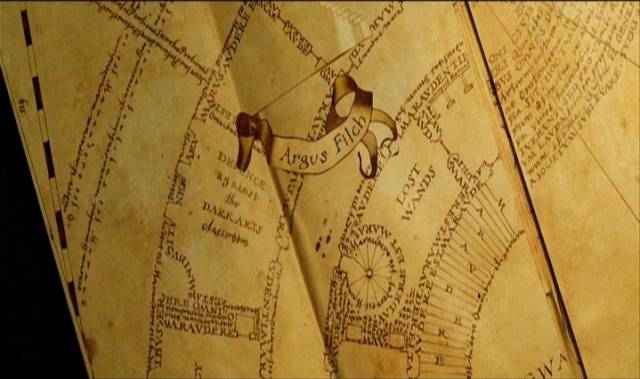
\includegraphics[width=\textwidth]{./img/marauder.jpg}
    \caption{Morceau de la carte du Maraudeur tirée du film}
    \label{marauder}
\end{figure}

Nous avons donc décidé de proposer une manière simple pour tout le monde de pouvoir s'orienter et retrouver des personnes dans les locaux de l'ISIMA au travers d’une application. Cette solution devra donc récolter l’ensemble des données sur les usagers de l’ISIMA et les reporter sur une carte qui sera bien sûr électronique. Nous voulons ainsi que chacun puisse sortir notre carte de sa poche pour retrouver un ami ou un collègue instantanément.

De manière générale, nous devons être capable de visualiser une carte de l'ISIMA, mais également de pouvoir trouver facilement une personne, un bureau ou une salle de cours. De plus, il serait intéressant de pouvoir localiser n'importe quelle autre personne sur la carte en temps réel. Cette visualisation doit s'actualiser assez rapidement pour que la localisation de personnes soit la plus précise possible pour les utilisateurs.

Une fois cette solution éprouvée avec les bâtiments de l'ISIMA, nous pouvons penser l'étendre à n'importe quel autre bâtiment dont nous pouvons avoir les plans. L’intérêt ici étant de développer une preuve de fonctionnement du suivi de personnes dans un bâtiment qui plus est considéré comme étant très surchargé de signaux. Comme nous l’évoquions plus tôt ceci pourrait trouver différentes utilisations dans différents contextes comme par exemple le fonctionnement d’un hôpital, la surveillance d’une prison, l’évacuation d’un bâtiment. Avec l’avènement de l’open data, il y a aussi de nombreuses questions éthiques à résoudre vis-à-vis des informations récoltées et diffusées.

Il faut aussi se demander comment notre application va se positionner par rapport aux applications existantes. Pour ce faire nous allons maintenant aborder l’analyse de l’existant.


\subsection{Analyse de l'existant}

Nous ne nous attarderons pas dans cette partie sur la carte magique imaginée par J. K. Rowling mais nous allons plutôt voir les différentes applications existant autour de la localisation d’usagers.

Le premier exemple est celui des réseaux sociaux. En effet, avec leur avènement est arrivé aussi un moyen pour des grands groupes de récolter une masse importante d’information sur leurs utilisateurs : ce que l’on appelle le Big Data. Dans cette masse de données, il y a bien évidemment des données de géolocalisation. Celles-ci sont de plusieurs types : soit données, soit mesurées.

Les premières, dites données, sont les informations que l’utilisateur va donner de lui-même aux réseaux sociaux comme par exemple poster une photo d’une après-midi entre amis en spécifiant le lieu de la prise de vue. Cette information peut être légitimement utilisée puisque donnée par l’utilisateur mais cela ne représente pas une source fiable ni même précise. Même si cette information n’est pas fiable, les réseaux sociaux ont trouvé depuis 2014 une toute nouvelle utilisation à ce type d’information : l’aide aux personnes en danger. En effet, Facebook a développé un service nommé Safety Check \ref{fbsafetycheck} qui repère les personnes présentes à proximité d’une zone de danger que ce soit une catastrophe naturelle ou bien encore une action terroriste et leur propose de se signaler en sécurité auprès de leurs proches. Le Safety Check visible à la figure \ref{safety-check} est un bon exemple de localisation de personnes mais demande à ce que les personnes recherchées effectuent une action.

\begin{figure}[H]
    \centering
    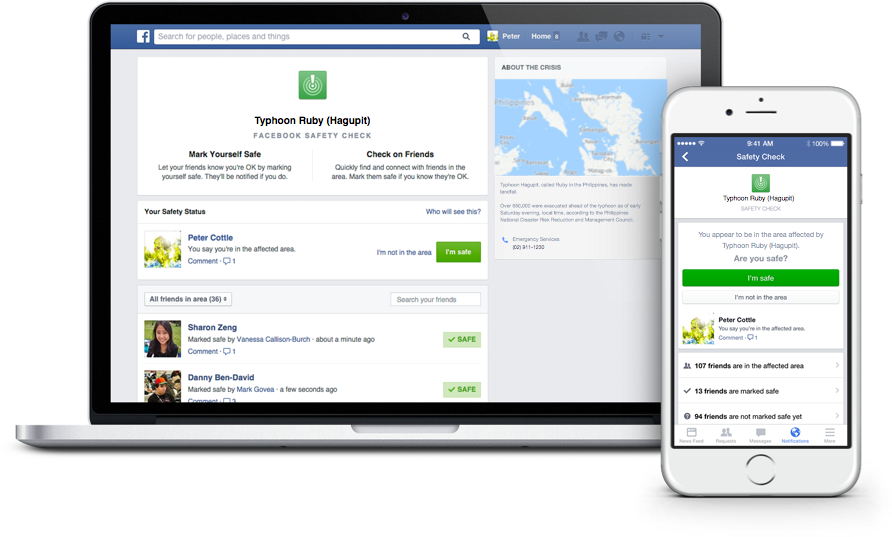
\includegraphics[width=\textwidth]{./img/safetycheck.png}
    \caption{Service Safety Check de Facebook}
    \label{safety-check}
\end{figure}

Le second type dit données mesurées représente toutes les informations que les réseaux sociaux récupèrent sur les appareils des utilisateurs. Cette récupération est rendue possible tout d’abord par l’existence de ces données. En effet depuis quelques années avec l’arrivée des smartphones et des objets connectés, la majeure partie des appareils électroniques possèdent des fonctionnalités de géolocalisation. Il est alors facile pour une application d’accéder à la position de son utilisateur. En général, l’appareil en question est un smartphone et se trouve très souvent au même endroit que son propriétaire, voire sur lui-même. On peut clairement constater la récupération de ces informations lorsque la localisation d’un utilisateur est associée directement au message qu’il poste ou bien encore sur les historiques. En effet, Google propose à ses utilisateurs d’accéder à tous l’historique de leurs déplacements \ref{bibgoogle} comme on peut le voir sur la figure \ref{google-maps}. Google récupère en permanence la position de utilisateurs afin de pouvoir fournir à la communauté des statistiques sur l’affluence de certains lieux, de demander des informations et photos sur les lieux en cours de visite ou bien proposer des services à proximité. Google arrive ici à localiser avec précision dans quel établissement une personne se trouve mais ne partage pas les données individuelles au reste de la communauté.

\begin{figure}[H]
    \centering
    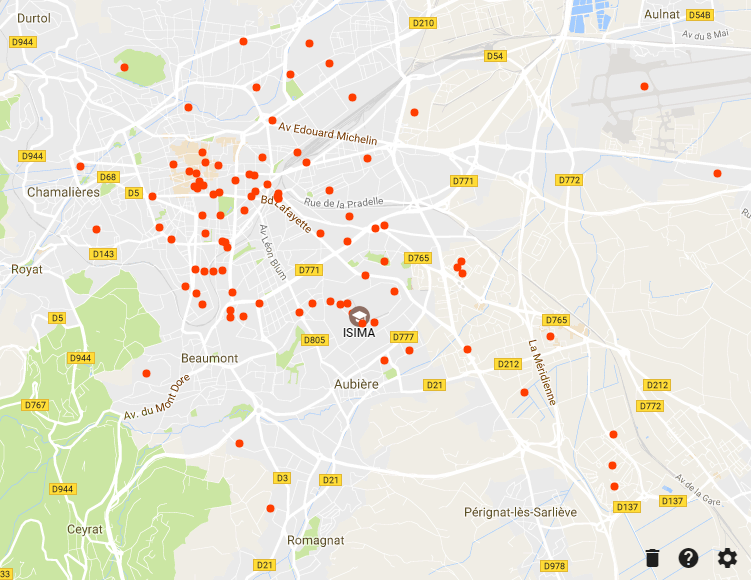
\includegraphics[width=\textwidth]{./img/googlemaps.png}
    \caption{Suivi des déplacements sur Google Maps}
    \label{google-maps}
\end{figure}

Les réseaux sociaux sont donc un acteur de premier plan dans la géolocalisation de personnes puisqu’ils disposent de nombreuses données sur le sujet mais ne diffusent qu’une fraction de celles-ci. Nous allons maintenant voir qu’il existe des services plus ouverts.

\subsubsection{Les services open data}

Dans les communautés de développeurs le phénomène open source qui consiste à partager librement les sources de ses propres programmes connaît beaucoup de succès. Sur cette base a émergé un nouveau concept : celui de l’open data. Comme son nom l’indique l’open data consiste à partager des données utiles récoltées.

Ces données sont le plus souvent fournies sous la forme d’un service web ou bien d’un fichier facilement découpable et analysable comme un fichier xml ou csv. L’intérêt est que ces données soient réutiliser par d’autres personnes en vue de concevoir un service plus consistant que des données brutes. Ainsi on donne aux développeur le moyen de concevoir des applications se basant sur de vraies données ce qui a pour effet de motiver l’innovation et la concurrence dans un domaine.

Un des exemples les plus connus en France et qui rejoint notre projet est celui de la société Keolis qui gère le service de transport en commun de la ville de Rennes. Cette société a décidé depuis sept ans déjà d’offrir au grand public des données utiles sur son activité de transport dans la ville de Rennes. En outre, Keolis a équipé ses bus de balises gps et partage en temps réel la position des bus des différentes lignes \ref{stardataexplore}. Il y a deux avantages à cette ouverture pour Keolis : la communauté des développeurs peut concevoir d’innombrables applications reposant sur des données sans cesse renouvelées et ainsi disposer sans efforts des meilleurs services mobiles en matière de transport en France. En effet, en comparaison d’une ville comme Clermont-Ferrand où les applications de transports reposent sur les horaires fixes décidés en début d’année, la ville de Rennes propose une application souple qui s’adapte même aux retards individuels de chaque véhicule.

Comme on peut le voir sur la figure \ref{rennes}, la flotte rennaise peut être localisée à tout instant.

\begin{figure}[H]
    \centering
    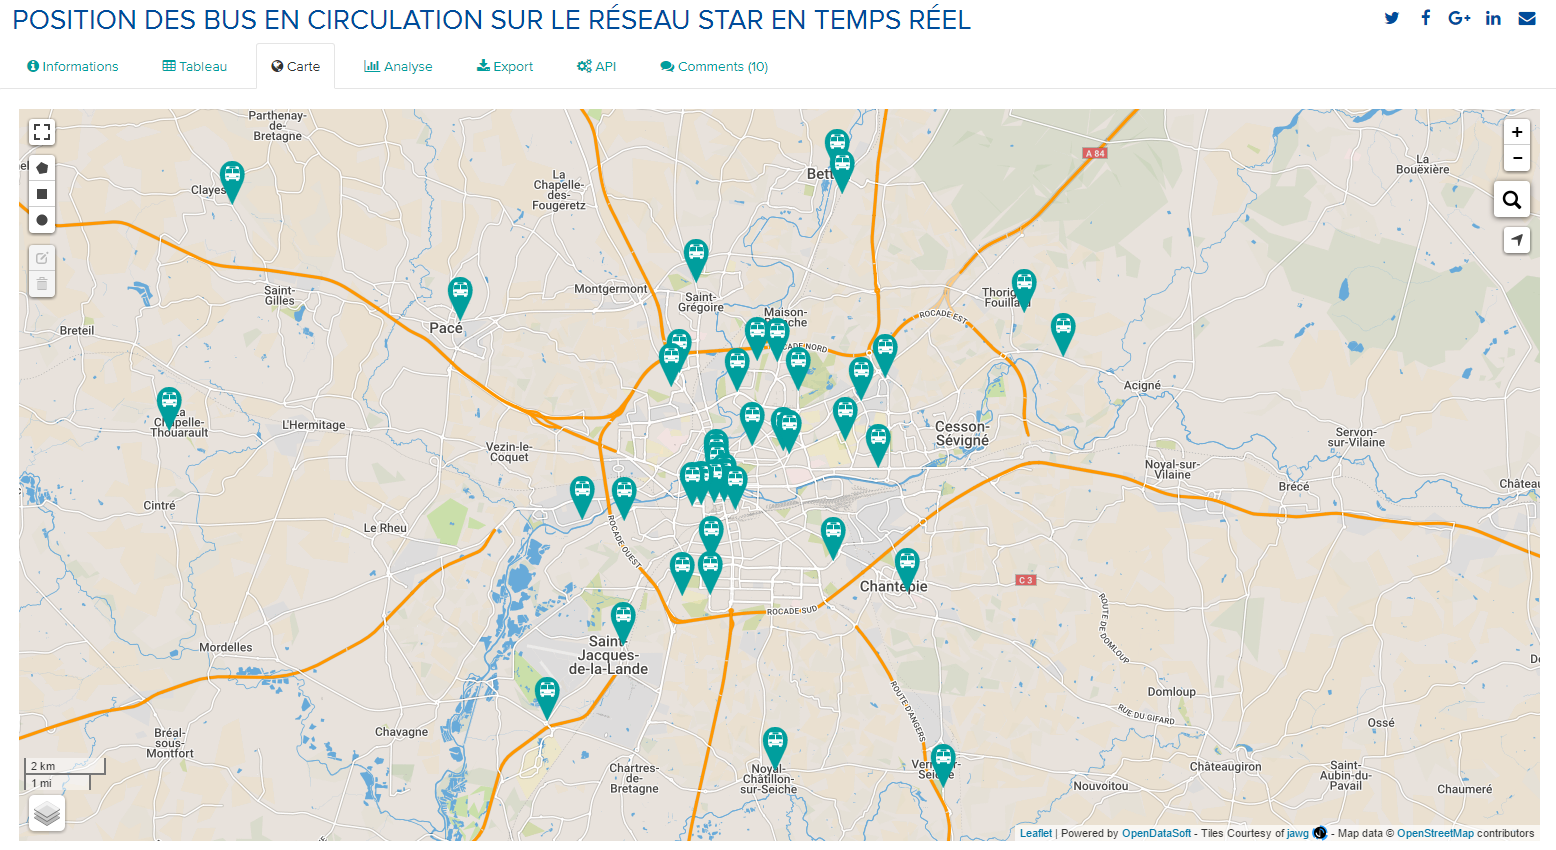
\includegraphics[width=\textwidth]{./img/rennes.png}
    \caption{Localisation en temps réel des bus de la ville de Rennes}
    \label{rennes}
\end{figure}

Dans ce cas, il est vrai que l’on ne parle pas de localiser directement des personnes mais des véhicules. Cependant des problèmes similaires se posent et se sont posés à commencer par la protection de l’identité. En effet, le service web proposait initialement d’obtenir pour chaque bus son numéro d’identification mais ceci permettait de suivre un véhicule en permanence. On peut imaginer beaucoup de choses sur l’utilisation d’une telle information mais fort heureusement celle-ci a été retirée puisqu’elle n’apportait rien de plus aux usagers.

Il y a donc possibilité de produire des applications qui donnent accès à des positions en temps réel au grand public mais celles-ci posent vite des problèmes d’éthique et légaux. Nous allons donc voir les applications réelles qui existent sur la localisation de personnes.

\subsubsection{Les applications similaires}

Dans la plupart des recherches effectuées, on trouve des dispositifs électroniques permettant de suivre une personne dépendante comme un enfant, une personne âgée ou handicapée.

Par exemple la société Geotek propose à ses clients des boitiers GSM permettant de localiser une personne \ref{bibgeotek}. Ils proposent leur utilisation pour les personnes dépendantes et même pour l’optimisation des déplacements d’employés dans une entreprise. Cette offre se rapproche un peu plus de notre projet mais s’en éloigne un peu dans le sens où elle nécessite l’utilisation de matériel supplémentaire et concerne la localisation de seulement quelques personnes auprès d’une seule personne.

En cherchant sur le Google Play qui est la plateforme officielle de téléchargement des applications Android on trouve quelques applications de localisation. Ces applications prennent bien souvent la forme de réseaux sociaux pour les soucis de confidentialité évoqués plus tôt.

Dans cette catégorie on peut parler de Find My Friends \ref{bibfindmyfriends} produite par Family Safety Production (figure \ref{findmyfriends}). Cette application propose des fonctionnalités intéressantes puisqu’elle permet de localiser ses amis qui possèdent l’application. Mais ce n’est pas tout, ils proposent aussi de pouvoir localiser les personnes qui n’ont pas l’application en envoyant juste un SMS à cette personne et si elle répond « oui » sa position s’affiche chez le demandeur. Cette fonctionnalité est très intéressante car elle permet de s’abstraire de l’application chez une partie des personnes.

\begin{figure}[H]
    \centering
    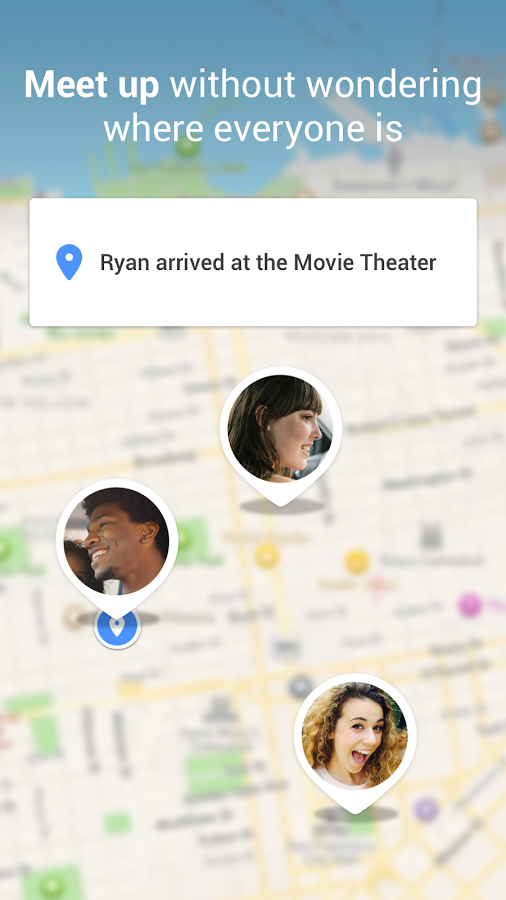
\includegraphics[height=8cm]{./img/findmyfriends.png}
    \caption{Application Find My Friends de Family Safety Production}
    \label{findmyfriends}
\end{figure}

Le point étant fait sur les applications existant nous allons maintenant définir plus précisément ce que nous souhaitons proposer au travers de notre application.


\subsection{Spécifications du projet}

Etant donné que peu de solutions sont disponibles sur le marché, nous avons choisi de partir de zéro et créer notre solution. Cela nous permet également d'avoir un contrôle total sur les données du projet, les diverses implémentations de fonctionnalités ainsi que la manière dont nous souhaitons utiliser notre solution.

La solution la plus évidente en termes de support de visualisation pour les utilisateurs est de leur proposer une application qu'ils pourront installer sur leur smartphone, PC, montre connectée ou encore tablette.

Afin de rendre cette application dynamique et de proposer un suivi de position d'utilisateurs en temps réel, il est convenu d'utiliser un service web. Ce service devra également pouvoir stocker des informations utiles aux utilisateurs, ce qui permettra également d'alléger le volume de données stockées sur leurs terminaux.

Nous allons donc détailler dans la suite les principaux éléments que nous voulons produire pour donner une vision de l’objectif final que nous souhaitons atteindre.

\subsubsection{Architecture}

Tout d’abord nous souhaitons fournir un service à un groupe de personnes plutôt important : nous avons donc besoin d’une architecture qui puisse gérer plusieurs utilisateurs sur une même application. L'architecture choisie pour organiser notre solution en est une de type client-serveur comme elle peut être décrite sur la figure \ref{architecture}.

\begin{figure}[H]
    \centering
    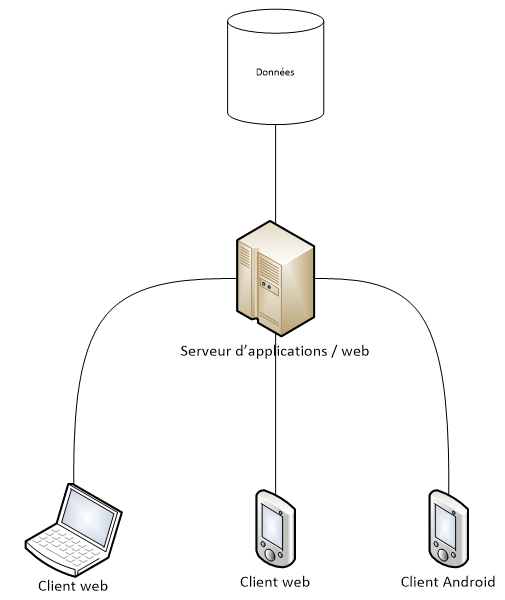
\includegraphics[height=10cm]{../infrastructure.png}
    \caption{Architecture générale de la solution}
    \label{architecture}
\end{figure}

Nous pouvons donc observer sur cette figure un schéma tout à fait classique de système client-serveur qui nous permettra de dissocier le développement du service du développement des différentes interfaces utilisateur. Un intérêt majeur est de pouvoir faire évoluer un des clients sans que cela n’impacte le cours de vie des autres projets reposant sur le service et le service lui-même.

Pour ce faire nous allons donc développer un service web de type REST pour que différent client, illustré dans notre projet par un client Android, puissent l’utiliser avec un minimum de contraintes. Les évolutions du serveur et du client n’auront donc pas d’impact l’un sur l’autre sauf bien sûr sur les modifications de l’interface. Si jamais un problème se déclarait dans la conception d’une partie nous comptons sur notre système d’intégration continue pour jouer le rôle de garde-fou en contrôlant le code versionné.

Nous allons maintenant aborder en détails les objectifs fixés pour chacun de ces éléments.

\subsubsection{Partie serveur}

Le serveur est le point reliant tous les clients et possèdent différents services mais la partie centrale est celle du service web. Le serveur doit être capable de répondre aux différentes connexions et requêtes des utilisateurs se connectant depuis l'application Android ou depuis tout autre client. Un service web n’est autre qu’un ensemble de services distants disponibles sur internet, ils peuvent permettre de récupérer des données ou bien d’effectuer des traitements spécifiques. L’intérêt est que le mode de communication avec un service web se veut standard ce qui permet à des utilisateurs de topologie différentes de le consommer.

Le serveur sera un service web de type \textbf{REST} c’est-à-dire qu’il sera capable de répondre à des requêtes se basant sur les protocoles web comme http dans un format standardisé, le JSON.
Le serveur disposera des fonctionnalités minimales suivantes :

\begin{itemize}
    \item un système d’authentification afin de valider l’identité des utilisateurs ;
    \item un service de collection des positions des utilisateurs ;
    \item un service d’obtention de la liste des personnes connectées ;
    \item un service de récupération de la position actuelle de l'utilisateur connecté ;
    \item un système de connexion/déconnexion des utilisateurs.
\end{itemize}

Ces fonctionnalités seront essentielles pour le fonctionnement de base de l'ensemble de la solution. Par la suite, des fonctionnalités supplémentaires pourront être ajoutées dans l'application, comme par exemple :

\begin{itemize}
    \item un historique des positions ;
    \item un service de calcul d'itinéraire entre deux positions dans le bâtiment ;
    \item un service de partage de position (par sms, mail, etc.).
\end{itemize}

Pour stocker les diverses informations utilisateur (login, position), nous avons convenu d'utiliser une base de données qui s'interfacera directement avec le service web.

L’ensemble devra donc être disponible sur une machine atteignable sur internet et devra avoir une haute disponibilité. C’est pourquoi il n’est pas concevable de le déployer sur un ordinateur personnel. Deux solutions s’offrent donc à nous :

\begin{itemize}
    \item l’utilisation d’une machine dédiée autogérée ;
    \item la location d’un IaaS ou CaaS (Infrastructure/Container as a Service).
\end{itemize}

La première solution consiste à utiliser une machine personnelle connectée en permanence à internet depuis notre domicile et la seconde à louer un service chez un fournisseur comme Amazon ou Google qui pourrait soit être une machine virtuelle Linux soit un conteneur d’applications. Le format aaS est à privilégier pour des raisons de performances et de disponibilité mais nous verrons que des soucis de budget nous ont conduit à opter pour la première solution.

Nous avons fait le tour de ce à quoi devra ressembler le serveur, abordons maintenant la question du client.

\subsubsection{Partie Android}

La seconde partie de ce projet concerne le client qui sera une application Android mais qui pourrait tout aussi bien être déclinée pour iOS et Windows Phone. Cette application sera donc une interface entre l’utilisateur et le serveur et devra lui permettre de profiter des fonctionnalités minimales attendues par rapport à la carte du maraudeur de Harry Potter.

Les fonctionnalités majeures seront donc :

\begin{itemize}
    \item l’inscription ;
    \item la connexion-déconnexion ;
    \item l’envoi de sa position gps au service web ;
    \item la réception des positions gps d'autres utilisateurs connectés ;
    \item la visualisation en temps réel sur une carte des positions.
\end{itemize}

Ces fonctionnalités forment le noyau dur indispensable au niveau minimal de qualité de notre application. Des améliorations sont envisageables pour augmenter le niveau de service, ainsi l'application pourra évoluer et proposer :

\begin{itemize}
    \item une carte en version 3D ;
    \item une carte en version réalité virtuelle ;
    \item le partage de position ;
    \item l'ajout d'informations sur la carte (lieu / point de rdv).
\end{itemize}

La mise à jour des informations sur le client sera initiée par l’application qui effectuera une requête sur le serveur. Le serveur renverra les positions des utilisateurs connectés qui permet sa mise à jour chez les utilisateurs.

Le choix d'une application Android se justifie par plusieurs facteurs. Tout d’abord il existe une communauté très active et de nombreux documents autour de l’Android. Ceci est dû en grande partie que le marché est majoritairement composé de terminaux Android, il y a donc plus de travail. Enfin le langage Android se basant sur du Java il nous est plus accessible de partir sur cette plateforme plutôt que sur du iOS ou même du Windows Phone, de plus nous avons quelques notions en Android.

Les versions du framework Android qui seront supportées seront les version 11 et ultérieures pour fonctionner sur un maximum de terminaux. Toutefois la version de compilation sera la 25 afin de pouvoir profiter des dernières mises à jour du framework. Ceci est rendu possible grâce aux ressources de post-compatibilité Android (appcompat) qui apportent aux terminaux un peu anciens certaines des améliorations non-existantes dans leur version.

Nous allons maintenant aborder un aspect important dans le développement de ce projet : son intégration continue.

\subsubsection{Intégration continue}

Un des objectifs de ce projet est de mettre en place une intégration continue et un déploiement automatique. Pour ce faire, il est nécessaire d'avoir un serveur dédié à cela. 

L’intégration continue est un ensemble de pratiques de génie logiciel permettant d’assurer la qualité et la non-régression du code au fur et à mesure du développement. L’intégration continue se base sur un système de versionnage de code et pour chaque commit, le serveur d’intégration teste des critères de non-régression du code, se charge du build et potentiellement déploie le résultat, s’il est correct afin de disposer en permanence d’une version fonctionnelle.

Notre serveur d'intégration sera un serveur Travis CI puisqu'il gère à la fois le NodeJS et l'Android qui est une nouvelle fonctionnalité récemment ajoutée. Cela permettra contrairement à un serveur Jenkins de ne pas avoir à gérer un serveur mais juste à consommer un service en ligne.

Le déploiement dans le cadre de l’application Android ne se fera pas sur le Google Play mais sur GitHub Releases pour des questions de budget. Un apk, qui est le format des applications sous Android, sera déposé par le serveur d’intégration sur GitHub Releases.

Concernant le web service, il sera déployé sur son propre serveur avec une phase de copie, d’installation et d’exécution du service.

Nous avons donc vu à quoi notre solution vise à ressembler, nous allons maintenant développer notre stratégie de planification du travail.

\subsection{Organisation du travail}

L'organisation temporelle théorique du travail est décrite dans le diagramme de Gantt de la figure \ref{ganttinit}. Elle se veut assez simple et découpée en quatre phases :

\begin{itemize}
    \item la phase de lancement qui s’étend jusqu’à la rentrée des vacances de la Toussaint et comporte toutes les travaux d’analyse et de mise en place du projet ;
    \item la phase de développement basique qui s’étend jusqu’à début 2017 et concerne le développement des applications minimales du projet.
    \item la phase d’amélioration durant laquelle l’ajout d’améliorations supplémentaires sera fait à l’application de base ;
    \item la phase de finalisation comportant la préparation de la documentation autour du projet.
\end{itemize}

La première phase est celle qui se prête le plus à un travail commun, puis les phases suivantes ont été pensé de façon modulaire afin de pouvoir travailler indépendamment de l’autre sur chaque tâche. Nous verrons plus tard comment le déroulement du projet a eu lieu dans les faits et quelles modifications de planning ont été apportées.

Nous avons discuté des différents points caractérisant notre projet et les objectifs que nous souhaitions atteindre, nous allons maintenant expliquer comment nous nous y sommes pris pour la conception dans la section suivante.

\begin{landscape}
    \begin{figure}[h]
        \centering
        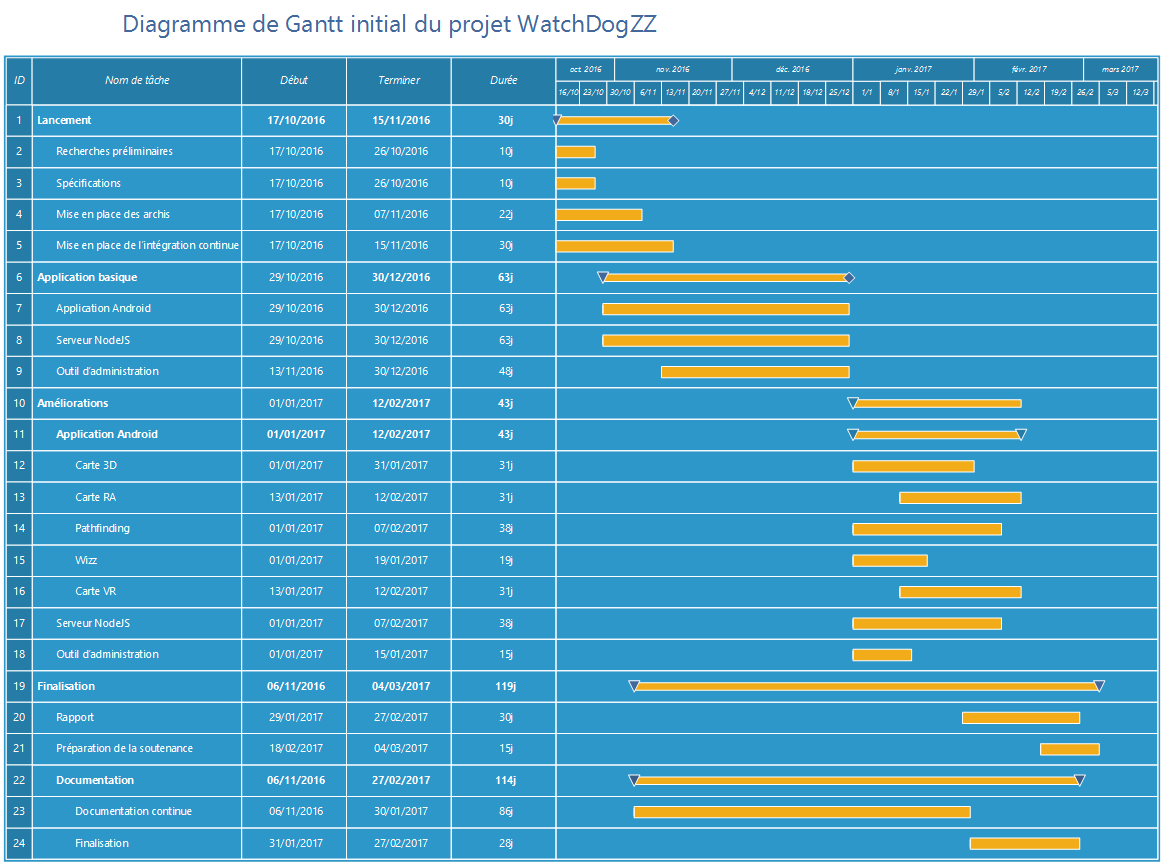
\includegraphics[height=\textwidth]{../gantt_initial.png}
        \caption{Diagramme de Gantt théorique}
        \label{ganttinit}
    \end{figure}
\end{landscape}

\section{Conception de la solution}

\subsection{Architecture de la solution}

    \subsubsection{Web Service}

    \subsubsection{Application Android}
Le développement du client mobile a suivi le schéma classique de conception d’une application Android. Pour rappel les objectifs initiaux majeurs de ce client étaient de pouvoir récupérer des données sur un web service, les exploiter, les afficher à l’utilisateur et enfin retourner des données au service en question. De façon général la solution Android s’organise en deux projets directeurs : les tests et l’implémentation de l’application. 

Il n’a pas choisi ici de faire du développement dirigé par les tests car la technologie Android était dans le cadre de ce projet une découverte et il aurait était hasardeux de définir des tests Java sur les concepts Android. Les tests ont donc ici vocation à valider les mécaniques métiers a posteriori ainsi que le bon fonctionnement et l’intégrité de l’application au fur et à mesure de l’ajout de fonctionnalités. La partie relative aux tests se subdivise en deux autres : les tests unitaires et les tests instrumentés. Les premiers sont plutôt classiques et permettent de tester les mécaniques métiers et de vérifier tout ce qui est mockable, autrement dit simulable. Toutefois, il y a certains aspects dans un programme Android qu’il n’est pas possible de mocker sans enlever l’intérêt du test. Nous parlons ici de fonctionnalités s’appuyant intrinsèquement sur le système Android comme les appels réseaux, le GPS, l’écran, etc. Il est nécessaire dès lors que l’on veut simuler une fonctionnalité Android même basique, de simuler tout un système Android. D’où l’intérêt de la deuxième catégorie de tests : les tests instrumentés. Ceux-ci vont être exécutés sur un émulateur Android directement afin de pouvoir tester dans notre cas les appels réseaux et l’utilisation du GPS.

Le projet de tests est donc un projet annexe venant en soutien au projet principal : celui du développement de l’application Android. L’ensemble doit gérer des données et les afficher, c’est pourquoi un modèle MVC semblait adapté. Le modèle MVC se compose de trois parties en interaction comme c’est visible \ref{mvc}. 

\begin{figure}
    \centering
    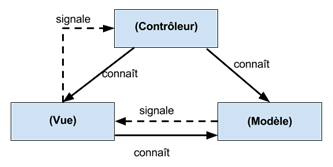
\includegraphics{./img/mvc.png}
    \caption{Patron de conception MVC}
    \label{mvc}
\end{figure}

Le modèle (M) représente les données traitées, dans le cas de l’application ce sont principalement les utilisateurs et leur position GPS. Les deux autres composants n’interagissent pas directement avec les données brutes mais on accès à l’API du modèle symbolisée par le gestionnaire d’utilisateur (UserManager). Le modèle gère donc tous les petits traitements bas niveau sur les données et les sert au reste de l’architecture selon les besoins.

Le contrôleur (C) s’occupe des interactions avec l’utilisateur, il doit pouvoir transmettre les commandes émanant de l’utilisateur aux autres composants.

\subsection{Fonctionnalités introduites}


\subsection{Je ne sais pas}
\section{Résultats}

Dans cette dernière section nous allons effectivement aborder le bilan de notre projet en présentant le résultat final obtenu et les diverses améliorations qui pourraient encore être faite sur ce sujet.

\subsection{La solution apportée}

Nous allons donc reprendre tour à tour les différents points présentés dans les parties précédentes et détailler point à point les fonctionnalités réalisées ainsi que la structure finale.

Nous avons donc réussi à atteindre nos objectifs minimaux durant ce projet et même à réaliser certains de nos objectifs supplémentaires. Nous avons réalisé un service web et une application Android qui sont tous les deux versionnés sur GitHub et intégrés en continu grâce à Travis CI qui nous permet de de valider l’intégrité de notre code et de déployer de façon automatique nos solutions. Les différentes versions majeures validées par l’intégration continue sont disponibles sur le site GitHub Releases et le service web est déployé sur une machine privée accessible depuis internet. Notre service web étant de type REST il pourrait être utilisé par différents clients en plus de l’application Android, mais nous n’avons développer que celui-ci par manque de temps c’est pourquoi il n’y a pas d’interface web comme on peut le voir à la figure \ref{archifinale}. Notre service est toutefois pleinement accessible depuis n’importe quel navigateur ou programme pouvant effectuer des requêtes http.

\begin{figure}[H]
    \centering
    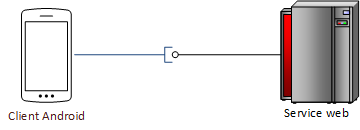
\includegraphics[width=\textwidth]{./img/archi_finale.png}
    \caption{Architecture finale simplifiée}
    \label{archifinale}
\end{figure}

L’architecture est donc assez simple et représente très bien le caractère binaire de notre projet : à savoir une partie serveur universel d’un côté et une partie client lourd de l’autre.

La dernière version de notre solution offre donc les fonctionnalités suivantes. Comme nous pouvons le voir sur la figure \ref{screen1}, nous avons mis en place un logo qui sert d’icône et d’image à notre produit, nous avons aussi une première activité ou vue, permettant la connexion des utilisateurs par le biais de leur compte Google. Comme expliqué dans la section précédente cette activité contacte dans un premier temps les services de Google pour authentifier l’utilisateur courant, pour se faire il faut envoyer l’adresse email, le mot de passe et la clé d’application de WatchDogZZ à Google qui va ensuite renvoyer un jeton en cas de succès. Ce jeton sera alors envoyé pour toutes les communications avec notre service.

\begin{figure}[H]
    \centering
    
\includegraphics[height=10cm]{./img/screen1.png}
    \caption{Logo et page de connexion de WatchDogZZ}
    \label{screen1}
\end{figure}

Cette première activité est un classique des applications connectées Android moderne et apporte un niveau souvent bien plus fiable de sécurité qu'un système d'authentification géré par le développeur où les failles peuvent vite devenir nombreuses (mots de passes non chiffrés en base, etc.).

Une fois cette phase d’authentification passée, l’utilisateur arrive donc sur l’activité principale de l’application : la carte de l’ISIMA. Cette carte en trois dimensions est une simple vue OpenGL où l’arbre de scène du Renderer a été réimplémenté afin d’obtenir les fonctionnalités de navigation et d’affichage voulues de la carte.

Comme on peut le voir sur la figure \ref{screen2}, les différents utilisateurs sont visibles sur la carte, symbolisés par de petites sphères colorées. Leur position se met à jour automatiquement toutes les secondes. Un bouton dans le coin inférieur droit de l’écran permet aussi de positionner des points d’intérêt sur la carte.

L’application dispose d’un menu glissant utilisable en tirant le menu depuis le bord gauche de l’écran. Ce menu donne accès aux différentes fonctionnalités ajoutées comme :

\begin{itemize}
    \item la carte normale ;
    \item la liste des utilisateurs ;
    \item la liste des points d’intérêt ;
    \item le partage de position.
\end{itemize}

Les autres items n’ont pas encore été implémentés, ils n’ont pas été jugés prioritaires en regard des autres fonctionnalités.

\begin{figure}[H]
    \centering
    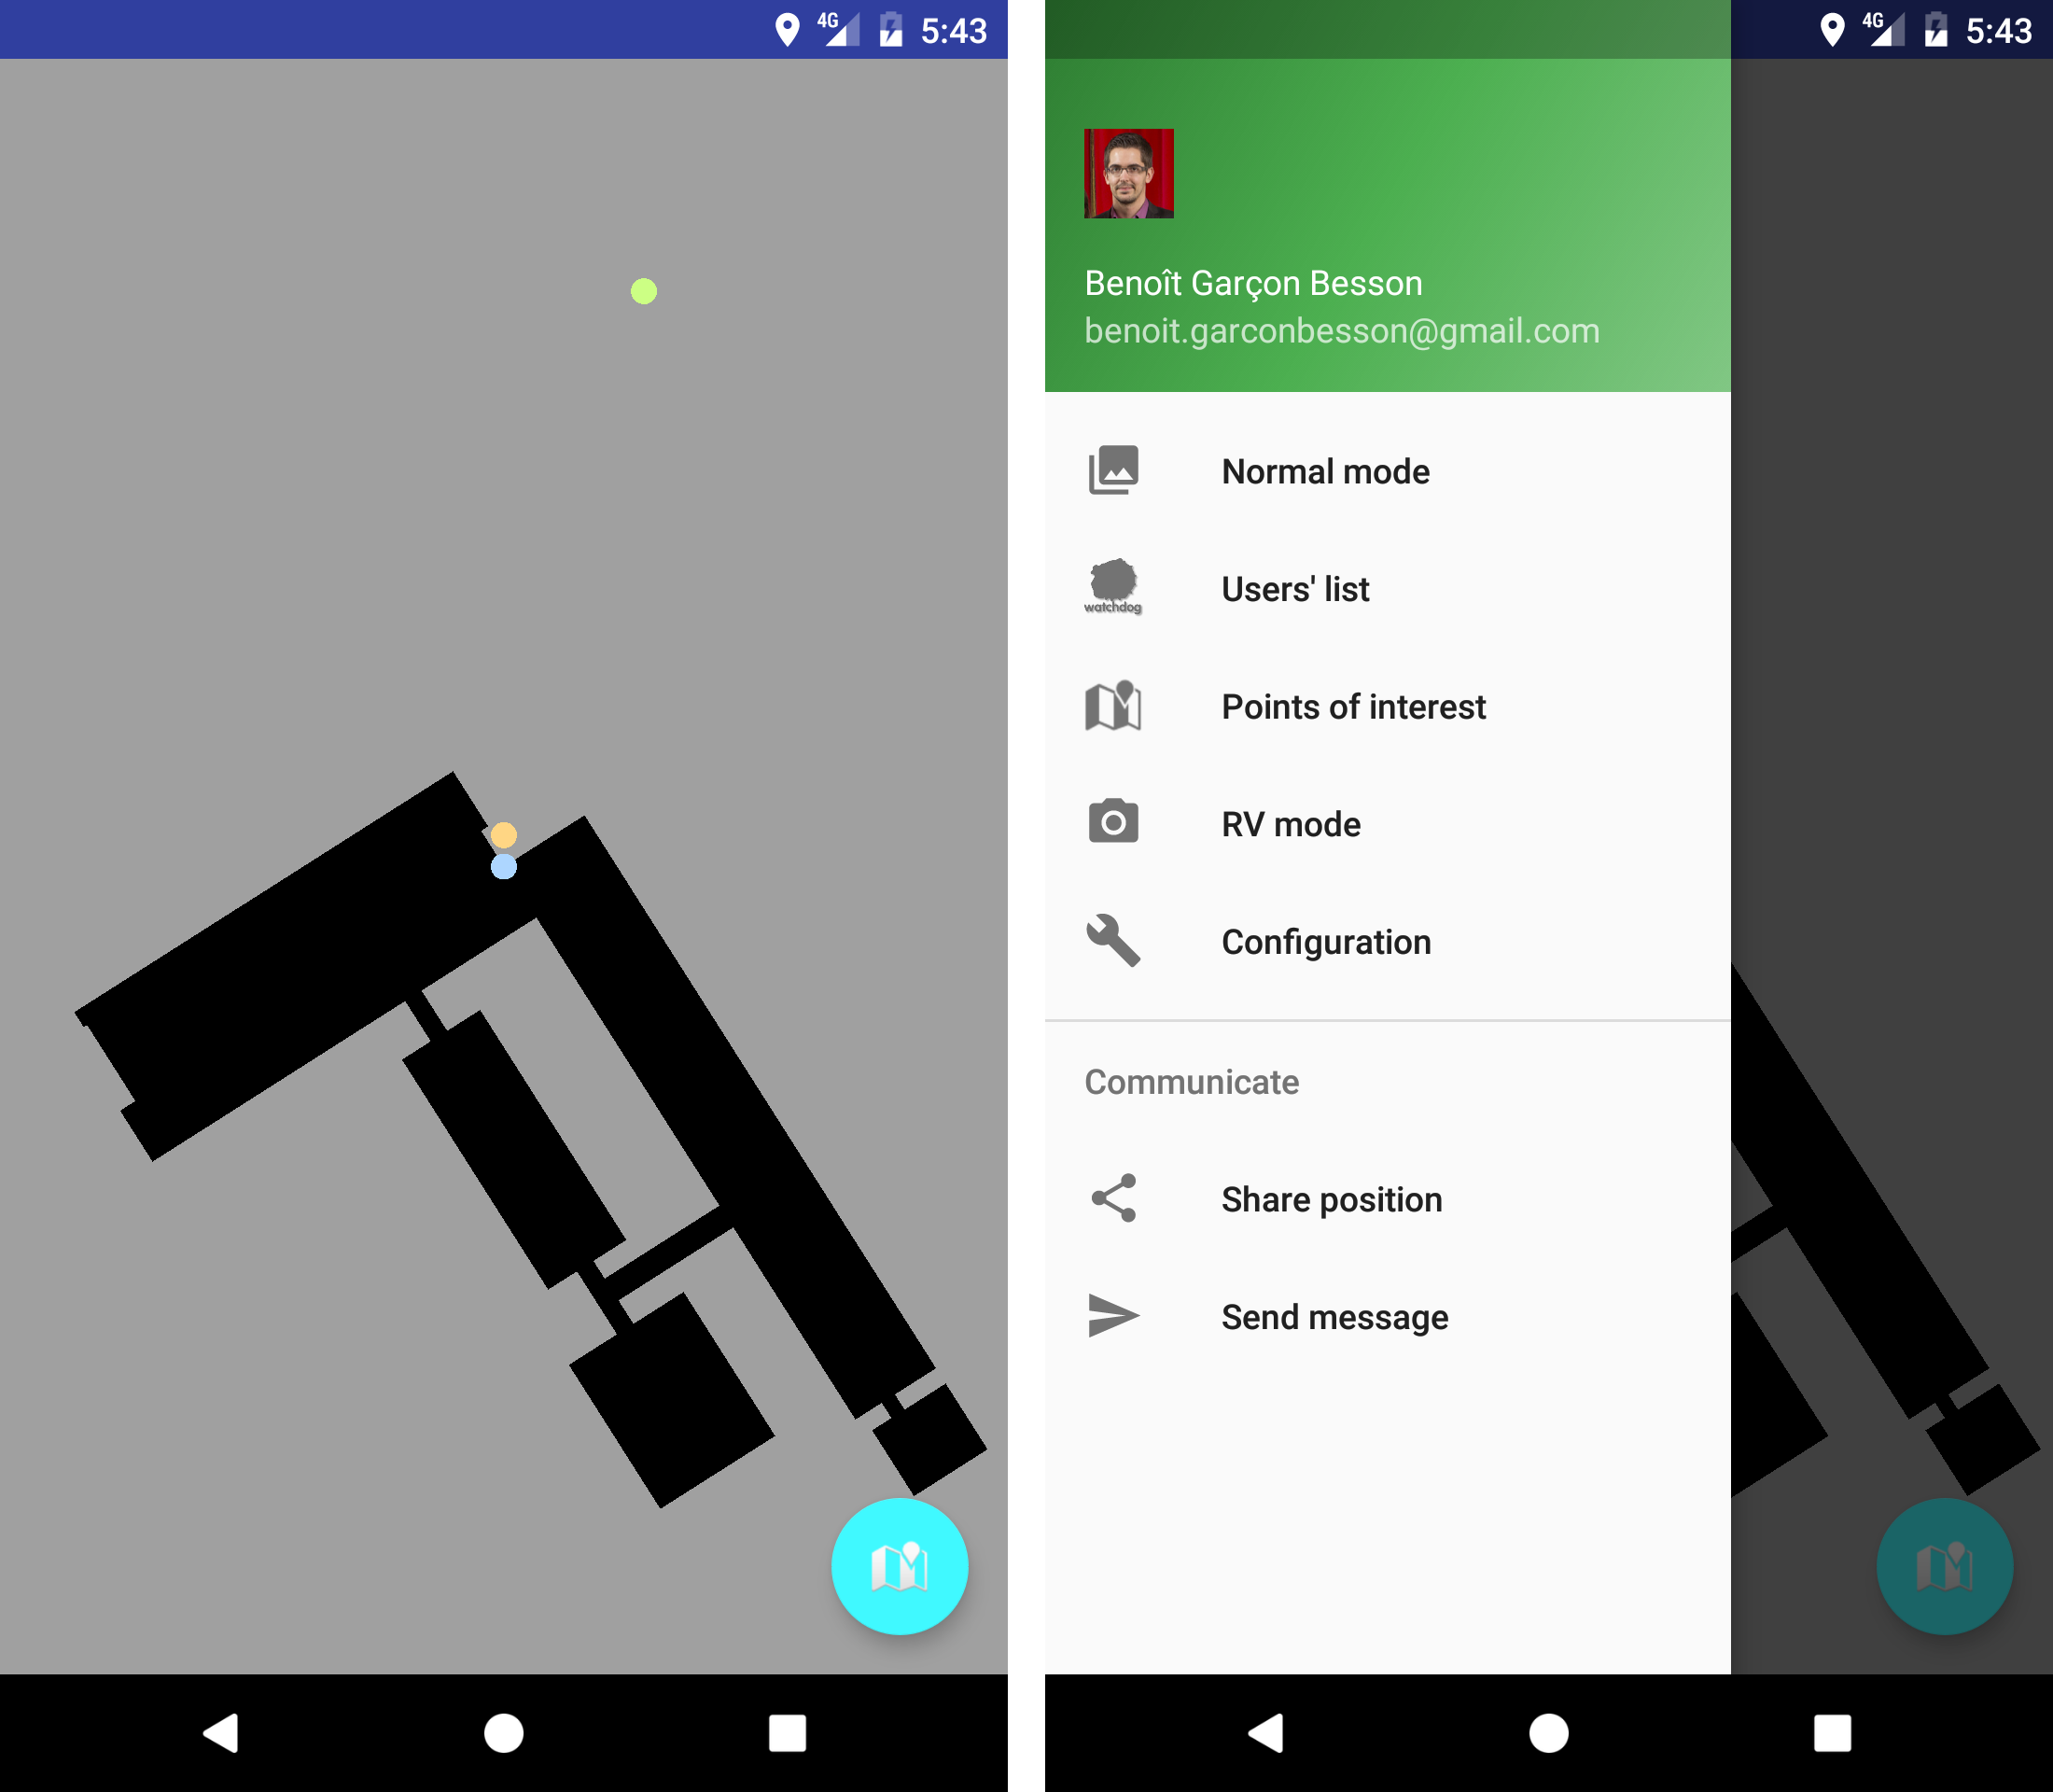
\includegraphics[height=10cm]{./img/screen2.png}
    \caption{Vue principale de la carte et menu glissant}
    \label{screen2}
\end{figure}

La liste des utilisateurs permet donc d’identifier plus aisément chaque utilisateur. On dispose comme sur la figure \ref{screen3} de la liste des utilisateurs avec leur photo et leur nom. 

\begin{figure}[H]
    \centering
    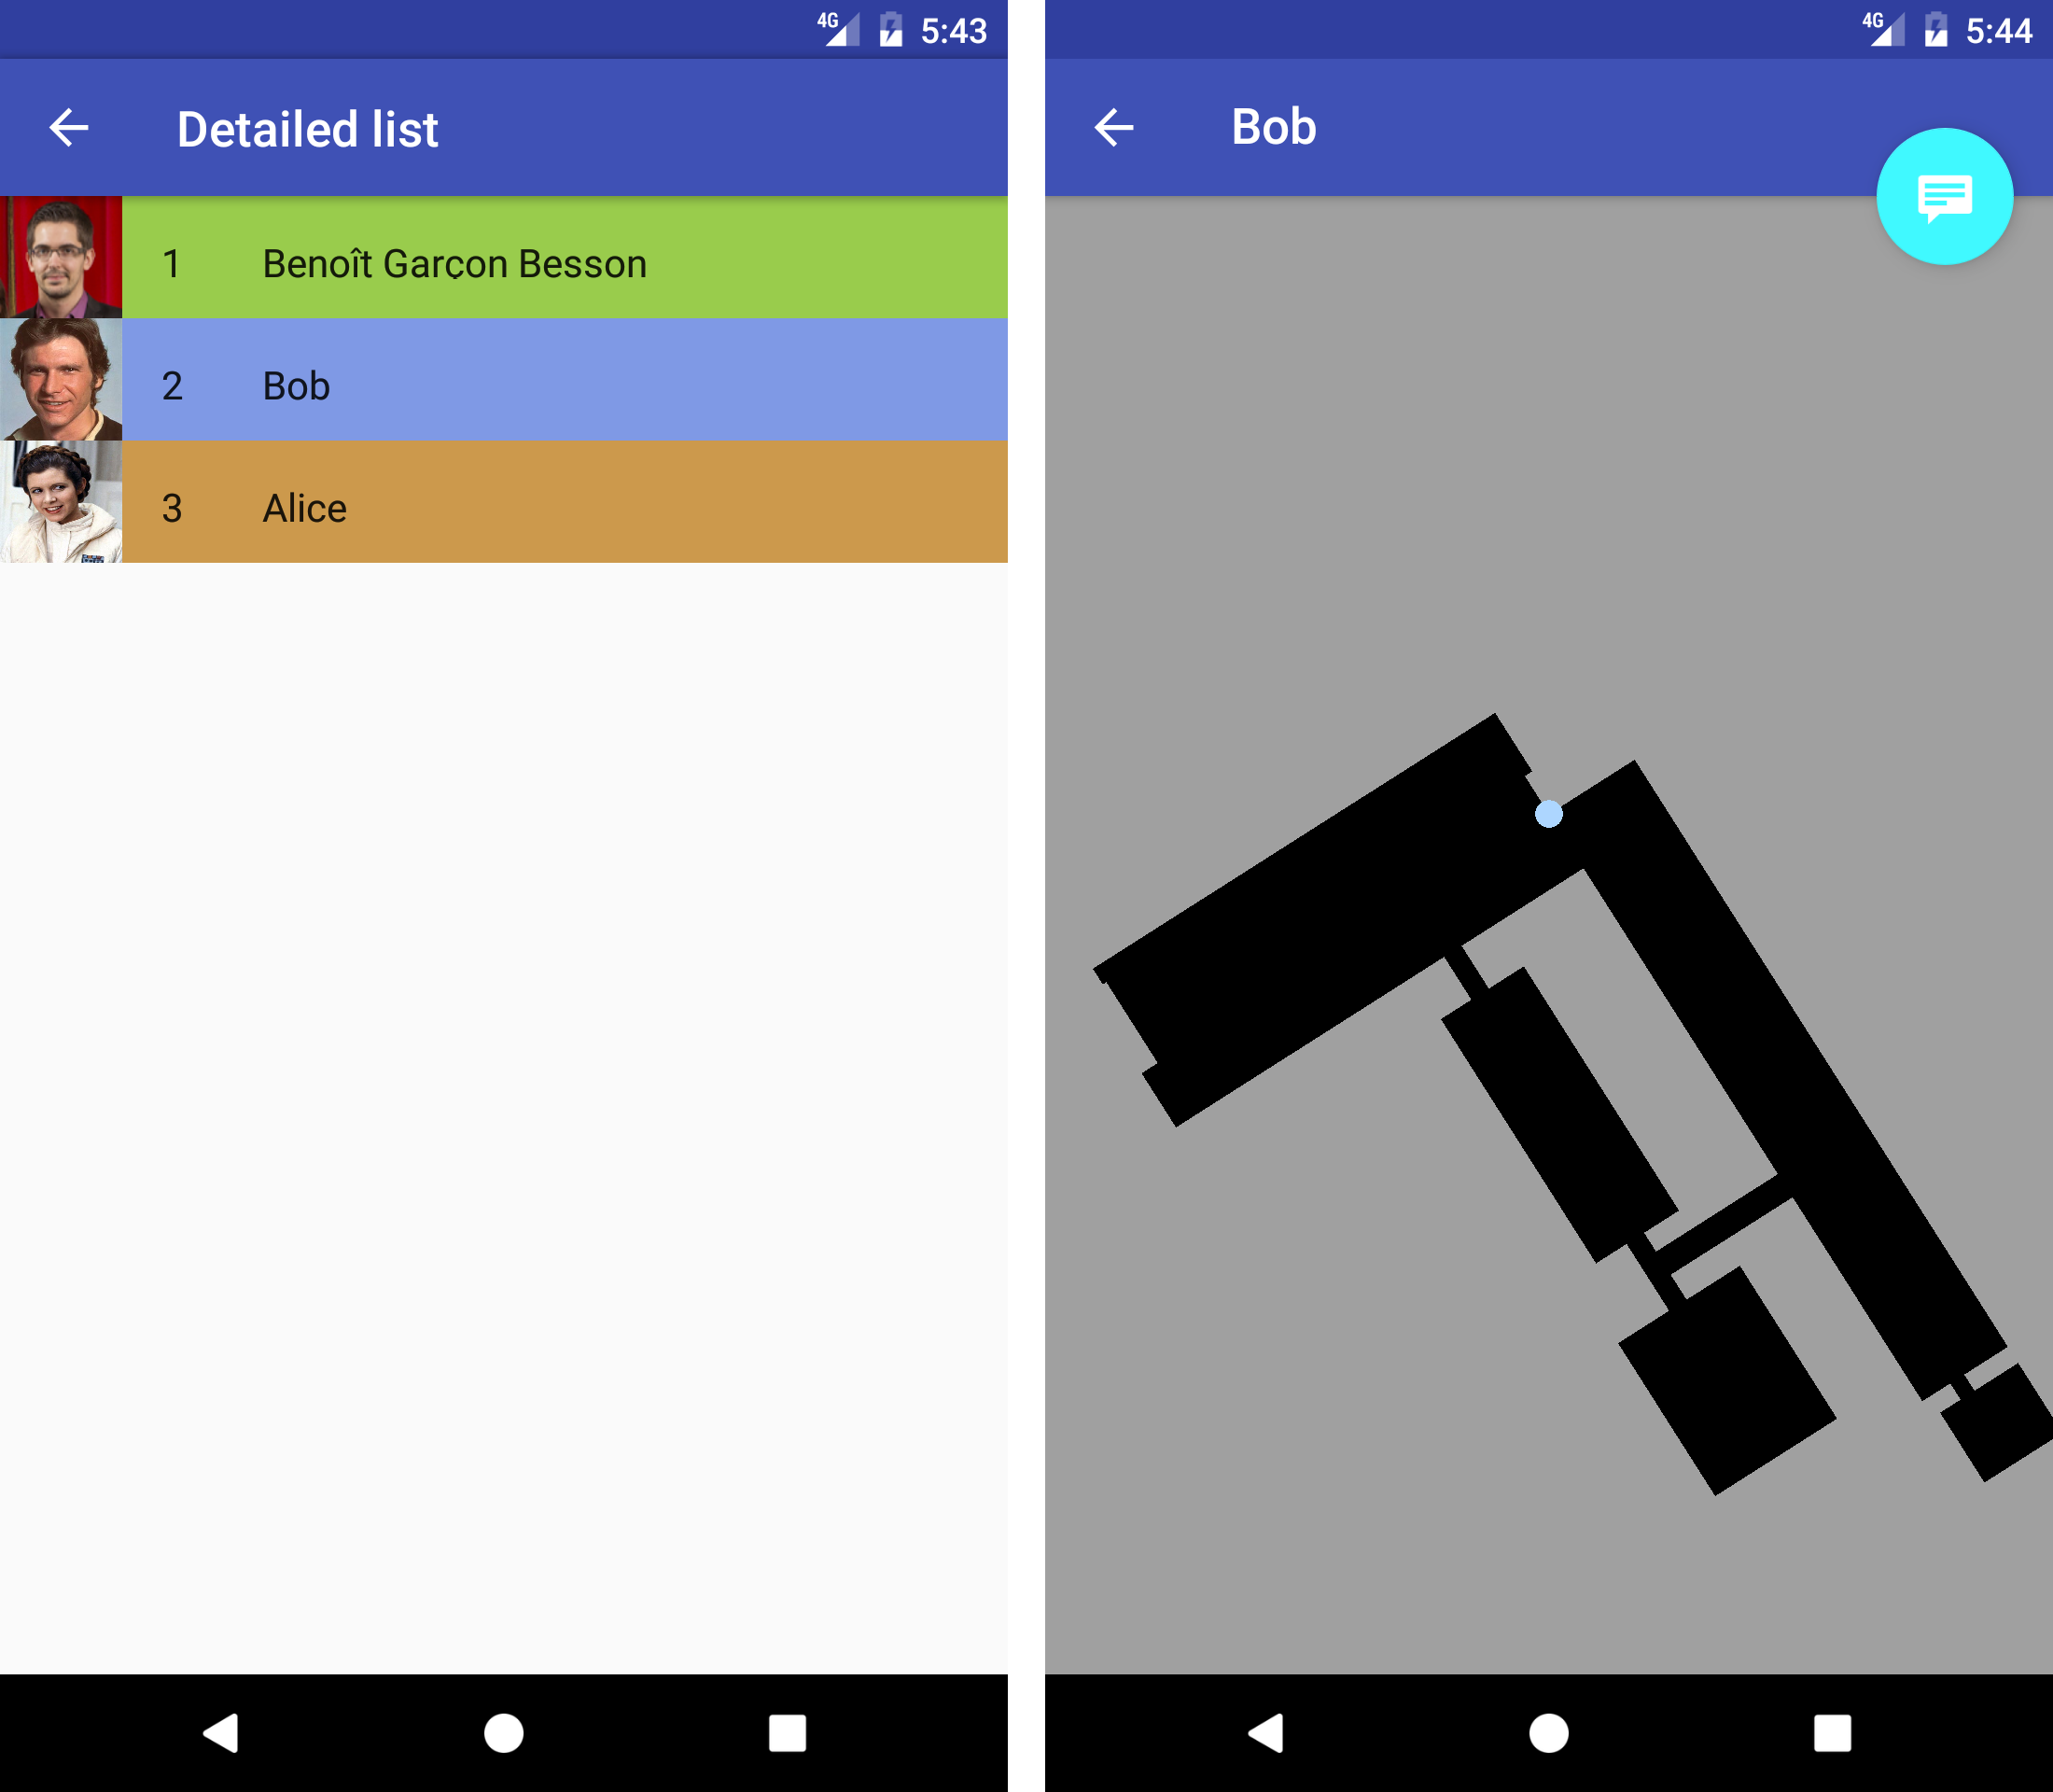
\includegraphics[height=10cm]{./img/screen3.png}
    \caption{Liste détaillée des utilisateurs}
    \label{screen3}
\end{figure}

La couleur associée à chaque utilisateur est issue du hashage de leur nom : ainsi leur couleur dans la liste est la même que celui de leur item sur la carte ce qui nous permet de les identifier. L’algorithme de hashage du nom est très simple et peut se traduire comme sur le code suivant.

\lstset{language=Java}
\begin{lstlisting}[caption=Hashage du nom en couleur]
int hash = label.hashCode();
r = abs((hash % 10)*255/10f/255f);	// calcul de la composante rouge
hash/=10;
g = abs((hash % 10)*255/10f/255f); 	// calcul de la composante verte
hash/=10;
b = abs((hash % 10)*255/10f/255f); 	// calcul de la composante bleue
\end{lstlisting}

De plus en sélectionnant un utilisateur dans la liste, on peut obtenir une carte simplifiée avec seulement le suivi de cette personne pour un suivi plus clair.

Pour en revenir aux points d’intérêt, leur ajout se fait comme dit précédemment par l’utilisation du bouton flottant au bas de l’écran. Cette action invite l’utilisateur à positionner le point vert à l’emplacement désiré et à valider ce placement avec bouton d’ajout. Cette nouvelle action lance un nouveau fragment permettant de nommer se point (figure \ref{screen4}).

\begin{figure}[H]
    \centering
    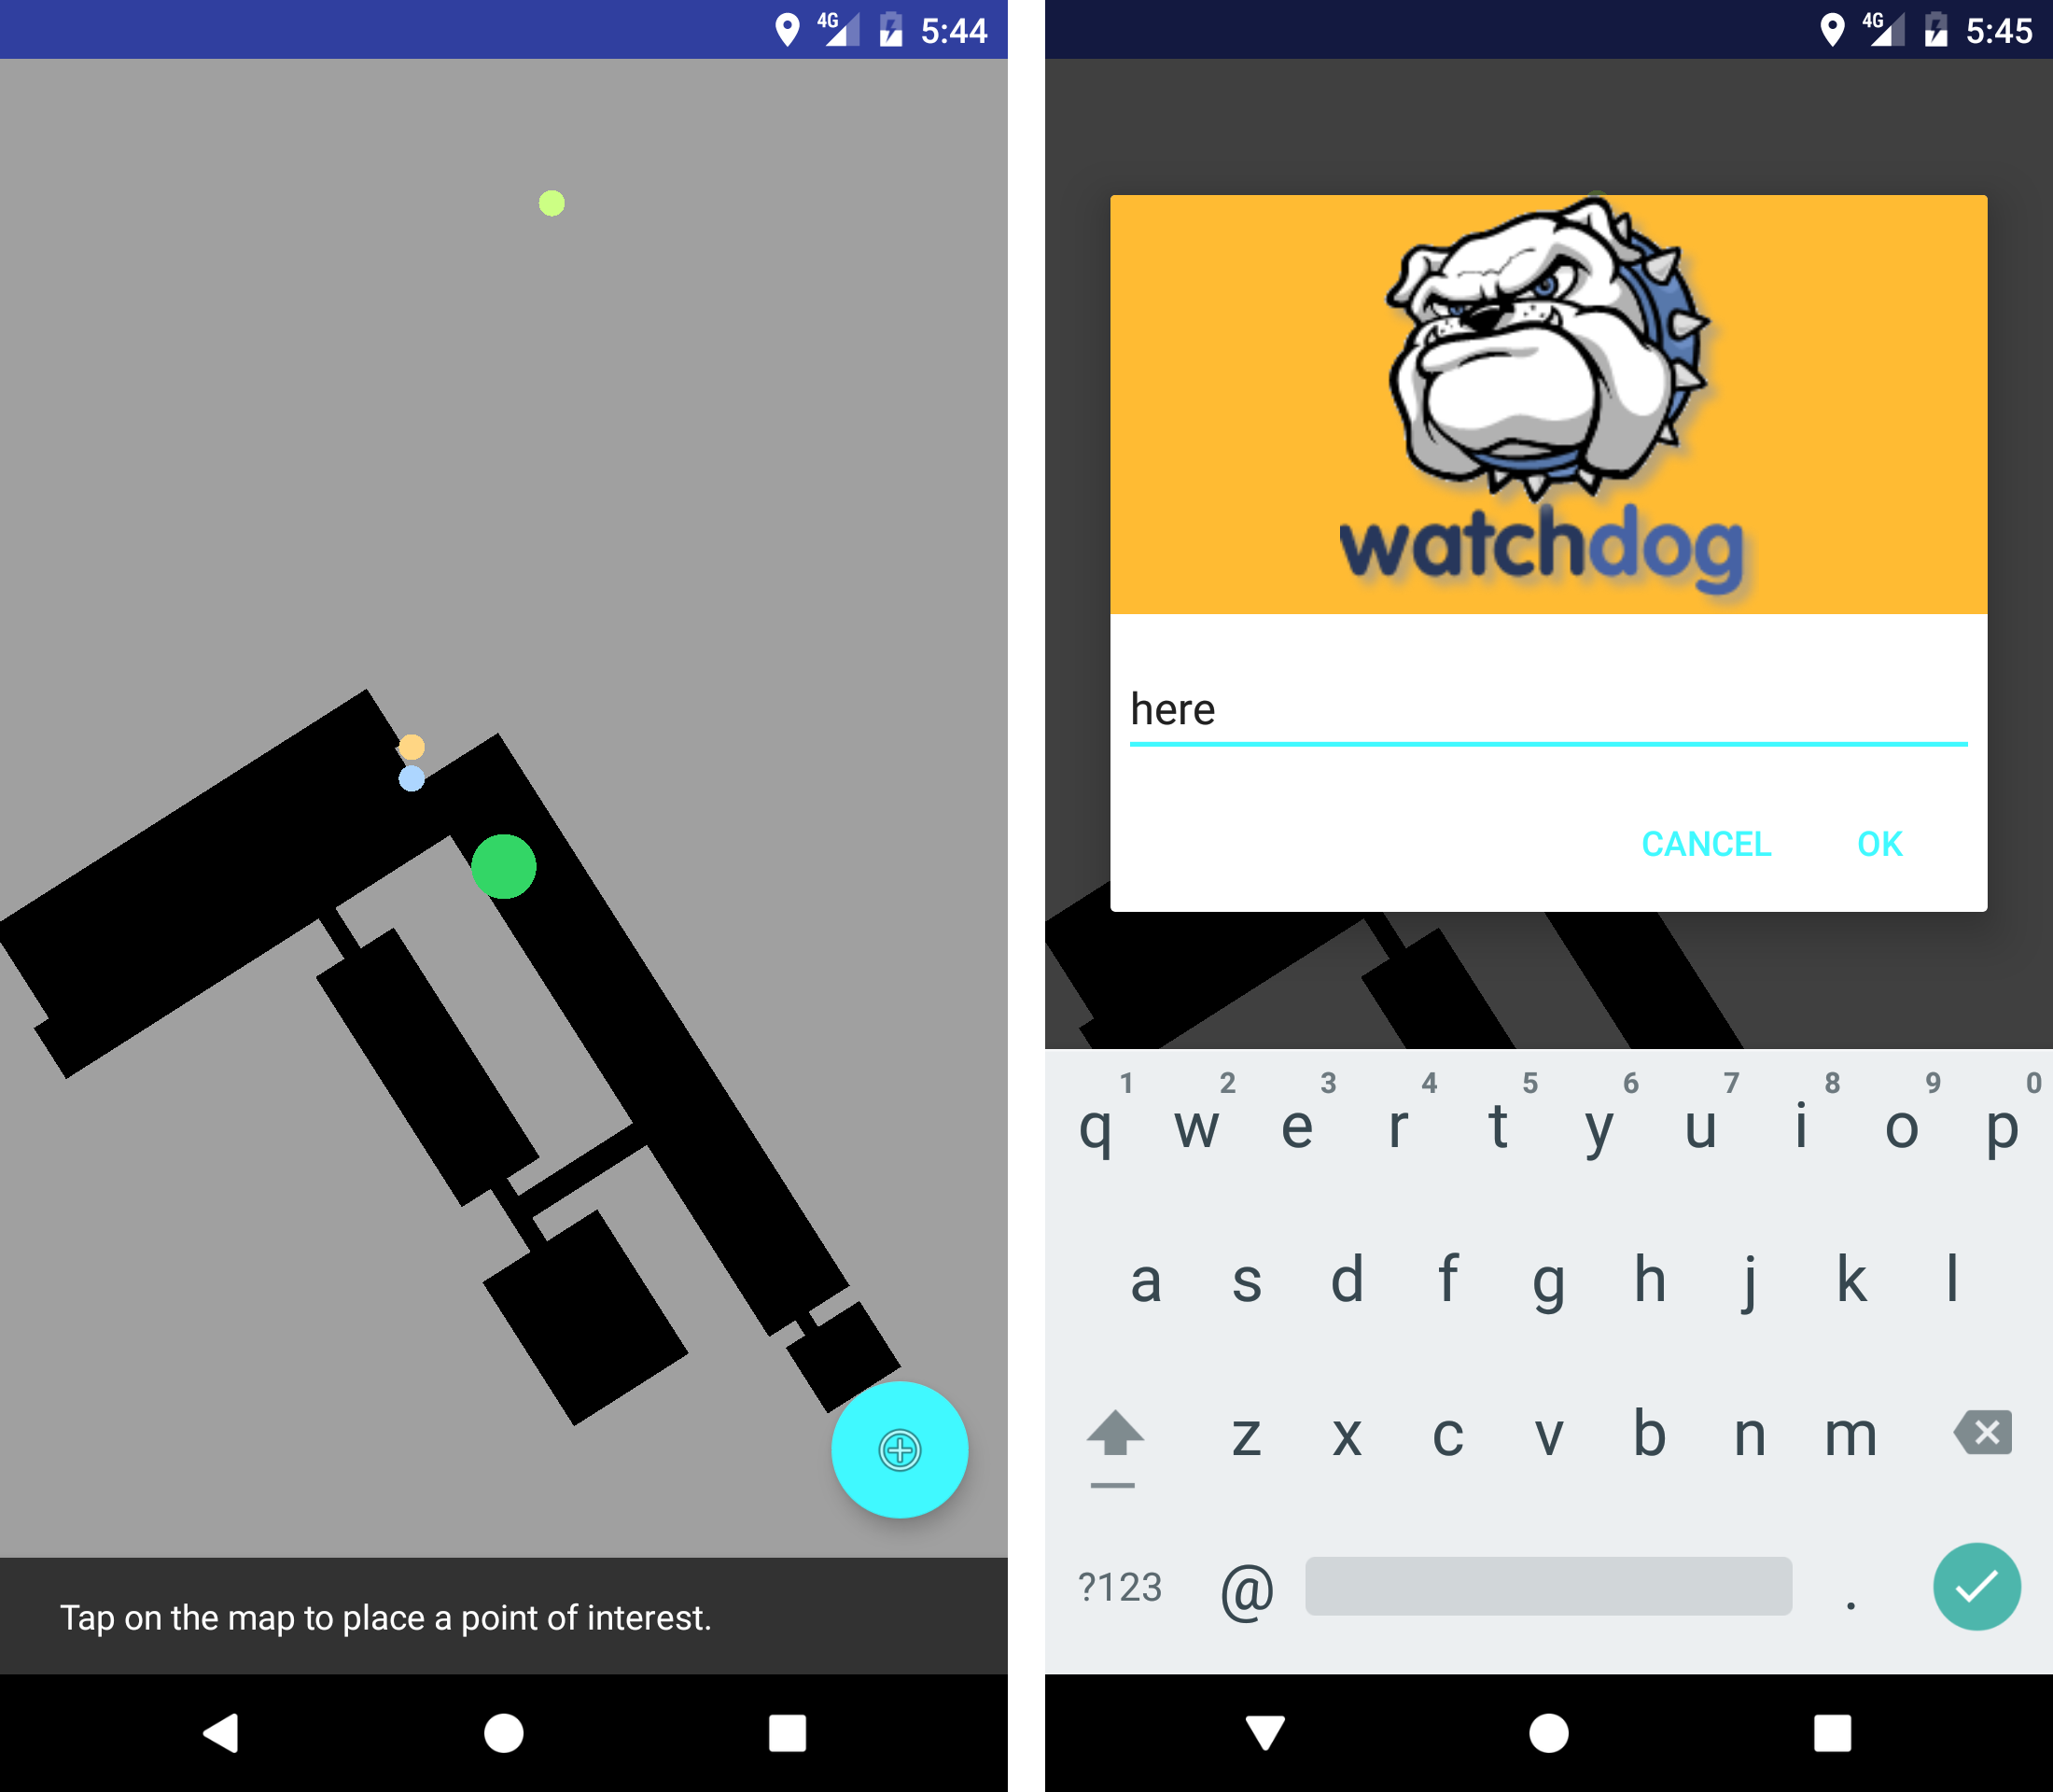
\includegraphics[height=10cm]{./img/screen4.png}
    \caption{Ajout d’un point d’intérêt}
    \label{screen4}
\end{figure}

Ce point est ensuite disponible dans la liste des points d’intérêt qui se base sur les mêmes principes que la liste d’utilisateurs. Comme on peut le voir sur la figure \ref{screen5}, une couleur est associée associer à chaque point par rapport à son nom et il est possible d’afficher le point sur la carte en le sélectionnant dans la liste.

\begin{figure}[H]
    \centering
    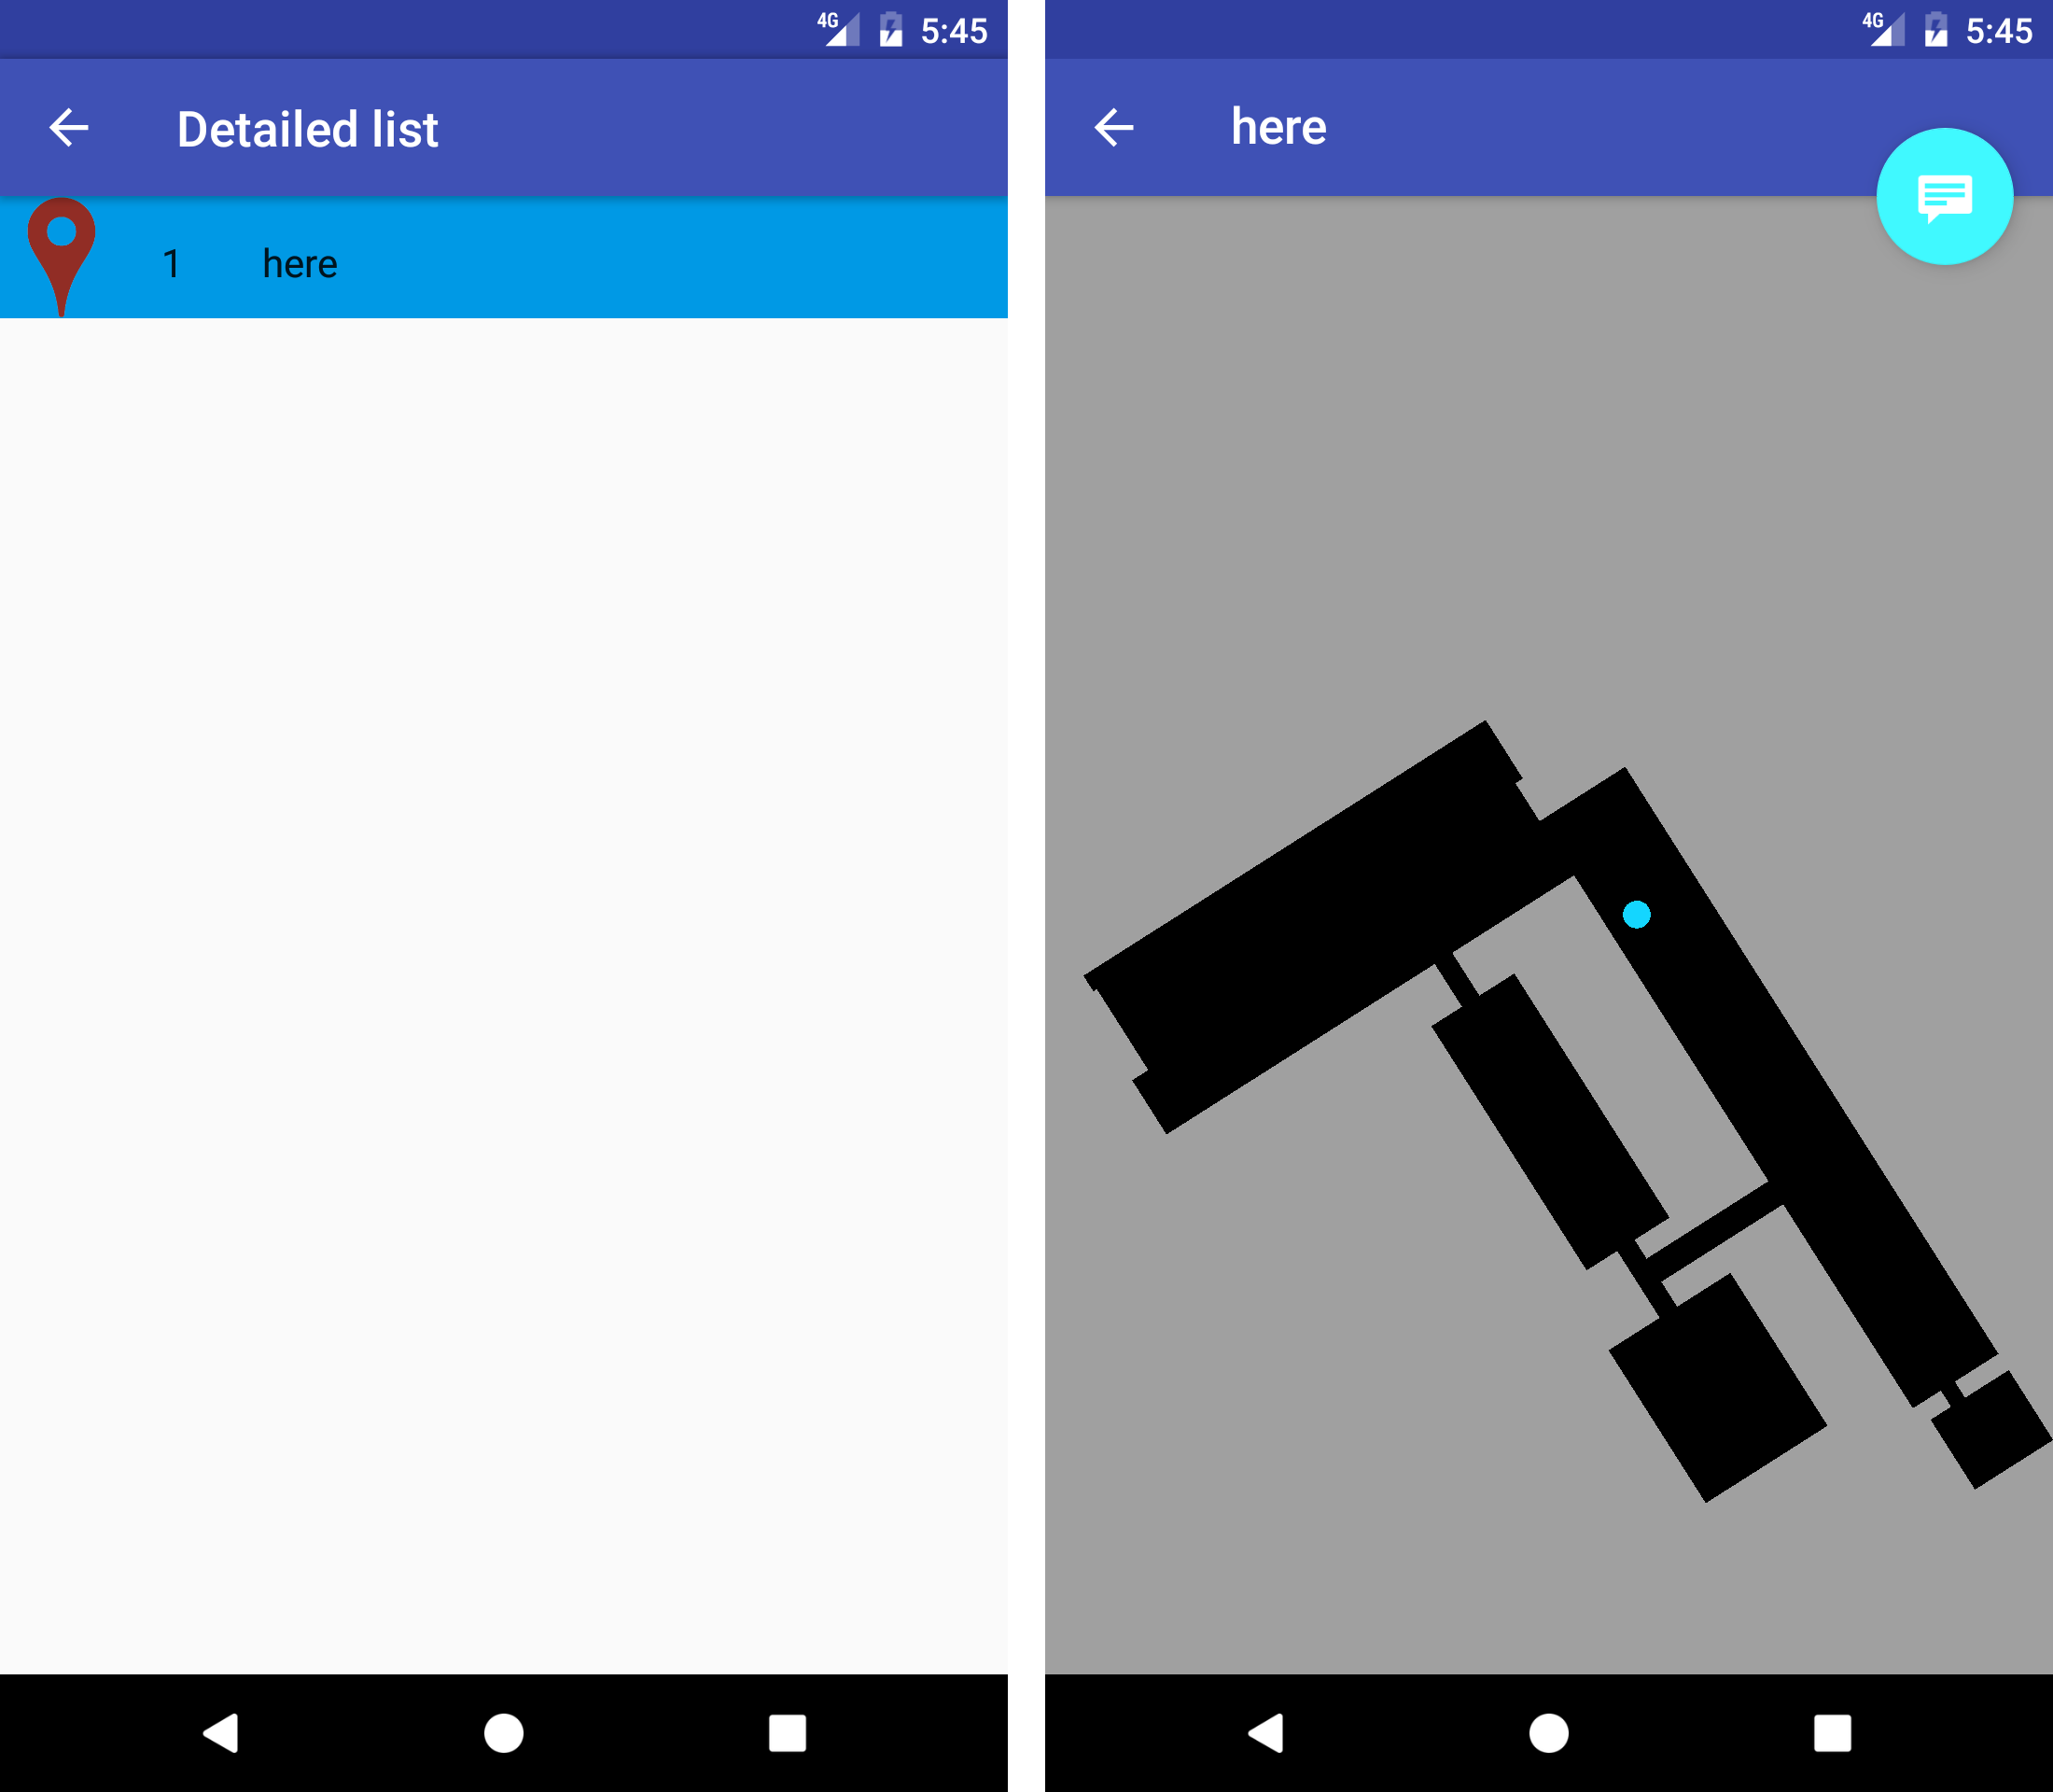
\includegraphics[height=10cm]{./img/screen5.png}
    \caption{Liste détaillée des points d’intérêt}
    \label{screen5}
\end{figure}

Toutes ces fonctionnalités nécessitent l’utilisation du serveur, mais la dernière, le partage de position est une fonctionnalité qui permet de s’affranchir du service web puisqu’il permet d’envoyer sa position à n’importe qui par n’importe quel moyen de communication. Ceci est rendu possible par les intents Android. Les intents sont des descriptions d’une action à effectuer et pouvant comporter des données nommées. Les intents sont produits par les applications pour être dirigées par le système Android vers l’application la plus capable d’effectuer l’action et en cas de choix multiple, la décision est donnée à l’utilisateur. Ainsi en produisant un intent devant envoyer le texte comportant notre position n’importe quel processus de type messagerie SMS, email ou autre peut l’envoyer : c’est au choix de l’utilisateur. On peut donc utiliser l’application même en cas de problème de communication avec le serveur.

Enfin concernant les communications avec le serveur, celles-ci sont sécurisées puisqu’elles utilisent le protocole https. Il a fallu pour ce faire créer un certificat pour le serveur enregistré auprès d’un service de certification et ensuite ajouter ce service de certification auprès des services de confiance de l’application. Au final ceci permet d’échanger avec le serveur toutes les informations personnelles nécessaires en garantissant la sécurité minimale.

Concernant les performances du service, elles semblent plutôt bonnes pour un nombre limité d’utilisateur. La position du terminal courant peut être récupérée à une fréquence au moins égale à la fréquence d’affichage sur le service gps et celles des autres ne nécessitent que quelques dizaines de millisecondes ce qui est plutôt convenable pour des appels réseaux répétés. Toutefois nous n’avons pas d’information sur le comportement de notre service à une échelle plus réaliste c’est-à-dire avec un nombre d’utilisateur représentatif d’une situation réelle. Nous aurions pu utiliser un outil comme Gatling pour effectuer des tests de performances et simuler l'utilisation de notre service par un grands nombre d'utilisateurs mais le temps nous manquait.

Nous avons vu toutes les fonctionnalités disponibles sur notre solution mais il en existe de nombreuses autres que nous n’avons pas pu développer et certains points pourraient aussi être améliorés.

\subsection{Améliorations possibles}

Bien que l'application WatchDogZZ soit à l'heure actuelle une application complète et répondant à nos attentes, ce projet reste un sujet très vaste et très ouvert sur lequel il est possible de faire énormément.

La première chose qui pourrait apporter un plus à WatchDogZZ serait une interface d’administration. Initialement nous avions prévu d’en développer une, mais devant la quantité importante de travail nous avons préféré resté concentré sur la partie client-serveur pure. En effet deux des objectifs de ce projet était de monter en compétences en Android et en développement de service web en NodeJS, le développement web d’un frontend ne nous aurait pas forcément apporté quelque chose dans ce cadre.

De plus il y a des détails de fonctionnement qui pourraient être améliorés comme par exemple l’utilisation du jeton d’authentification Google. Il est utilisé pour valider l’identité de l’utilisateur et ensuite transmis à chaque échange mais ce token n’est pas vérifier à chaque fois par le service auprès de Google. Ceci peut entraîner une faille de sécurité importante et devrait être corrigé avant une distribution de l’application. Concernant l’application Android elle aussi dispose d’une faille de sécurité puisque pour le moment elle est signée à l’aide d’une clé de debug au lieu d’une vraie clé de signature pour des raisons de simplicité de développement.

Ensuite, il y a quelques fonctionnalités que nous voulions ajouter mais elles n’ont pas été sélectionnées au cours des itérations. On peut citer par exemple :
\begin{itemize}
    \item la gestion des étages : actuellement, même si la carte est en trois dimensions, la composante altitude est uniformisée par soucis de calibrage ;
    \item l’utilisation d’une carte en réalité virtuelle avec la technologie Google Cardboard qui permet d’utiliser un smartphone comme un casque de réalité virtuelle en produisant deux images sur l’écran et en positionnant le smartphone à quelques centimètres des yeux de l’utilisateur ;
    \item le calcul d’itinéraire : l’application possède dans sa dernière version toutes les briques nécessaires pour faire un calcul d’itinéraire entre deux points (utilisateur ou intérêt) et l’afficher mais il reste à développer un algorithme de pathfinding manipulant nos données ;
    \item l’amélioration de l’interface utilisateur : l’interface est assez austère et n’est pas un produit commercialisable en l’état, il manquerait aussi à finaliser des micro-fonctionnalités générales comme le menu de configurations et des petits détails que l’on retrouve dans bon nombre d’application modernes, par exemple l’application a un système d’internationalisation qui n’a que deux langues, le français et l’anglais ;
    \item l’interception des SMS : nous aurions aimé pouvoir intercepter les SMS comportant un schéma spécial afin d’intégrer des informations provenant de sources multiples dans l’application. Par exemple ; lorsqu’un utilisateur partage sa position par SMS, si le destinataire possède l’application il pourrait être en mesure de l’afficher directement dans l’application sans savoir qu’il a reçu un sms avec des coordonnées gps brutes ;
    \item la communication entre usagers : il aurait été intéressant d’intégrer un service de messagerie à l’application pour pouvoir communiquer avec les autres usagers même si on ne dispose pas de ses coordonnées téléphoniques ;
    \item la gestion des logs du service : afin de pouvoir surveiller au mieux l’activité sur le serveur et pouvoir requêter des informations concernant une date, un utilisateur ou tout autre information utile ;
    \item un système de backup pour la base de données du serveur : en effet à l’heure actuelle aucune mesure de sauvegarde ni de restauration des données n’existe, ce qui ne serait pas tolérable sur un serveur professionnel.
\end{itemize}

Ce projet qui peut être perçu comme sans fin dispose d’énormément de possibilités d’évolutions et d’améliorations limitées seulement par notre imagination et notre budget.



%%% CONCLUSION %%%%%%%%%%%%%%%%%%%%%%%%%%%%%%%%%%%%%%%%%%%%%%%%%%%%%%%%%
\bookmarksetup{startatroot}
\addtocontents{toc}{\bigskip}
\newpage

\section*{Conclusion}
\addcontentsline{toc}{section}{Conclusion}

% header avec juste le nom de la section
\fancyhead[L]{Conclusion}
\fancyhead[R]{}

%%%%%%%%%%%%%%%%%%%%%%%%%%%%%%%%%%%%%%%%%%%%%%%%%%%%%%%%%%%%%%%%%%%%%%%%
% CONCLUSION
%%%%%%%%%%%%%%%%%%%%%%%%%%%%%%%%%%%%%%%%%%%%%%%%%%%%%%%%%%%%%%%%%%%%%%%%

Ce projet a donc été l’occasion de concrétiser au travers de l’application WatchDogZZ une idée personnelle. Nous avons pu développer une application complète reprenant les principes fondamentaux de la carte du maraudeur à savoir la géolocalisation d’usagers dans un établissement. A ceci de nombreuses fonctionnalités ont pu être ajoutées comme le partage de position, la gestion de points d’intérêts, etc.
Ceci est rendu possible par le développement combiné d'une partie serveur et d'un client. Le client est une application Android compatible avec tout dispositif (smartphone, tablette, télévision, etc.) disposant d’un système en version 12 ou supérieur. Le web service est basé sur le framework NodeJS couplé à une base de données NoSQL : MongoDB ; permettant la communication de données sécurisées par le protocole HTTPS. Ce sont donc des technologies émergente qui sont utilisées dans cette solution.

Au terme de ce projet tous les objectifs initiaux ont été atteints et de nombreuses fonctionnalités supplémentaires et de concepts originaux restent à développer. La taille du projet, ses spécifications et sa pluralité technologique en font un projet très complexe et demanderait beaucoup plus de temps pour être complet.
C'est pourquoi, en début de projet, il a été décidé de se concentrer sur les fonctionnalités de base du service que nous souhaitions implémenter, afin de disposer d'une base solide et évolutive.
Ceci a ensuite permis d’implémenter des fonctionnalités plus complexes dans des itérations de type "agile" en assurant qu’au terme du projet nous aurions une application fonctionnelle et répondant aux critères initiaux.
C'est ce cheminement qui a permis la création de la solution WatchDogZZ, fonctionnelle, et disposant de certaines fonctionnalités supplémentaires.

Ce projet nous a permis d’atteindre quatre objectifs que nous nous étions fixés. Les deux premiers étaient des objectifs techniques à savoir progresser dans la maîtrise d’Android et NodeJS afin d’augmenter nos atouts techniques sur le marché du travail. Le troisième était de produire une application dans la lignée des applications modernes c’est-à-dire interagissant avec des services web et proposant des interactions sociales. Enfin le dernier objectif qui fut proposé par notre tuteur et qui consistait à progresser dans nos méthodes de génie logiciel en utilisant de l’intégration continu et du développement agile. L’atteinte de ses objectifs relève d’une plus grande satisfaction que la production de la solution elle-même.

De nombreux axes d’amélioration et d’évolution restent encore ouverts pour notre projet. Tout d’abord, toutes les fonctionnalités auxquelles nous avons pensé n’ont pas toutes été implémentées comme par exemple la vue en réalité virtuelle de l’établissement ou encore le calcul d’itinéraire. Celles-ci restent facilement intégrables dans l’application qui possèdent tous les prérequis à leur intégration.

Du point de vue de la diffusion de l'application, deux points majeurs peuvent être améliorés. Le premier concerne la portabilité du client : en effet il n’est actuellement disponible que sur les appareils Android, un portage iOS et Windows Phone permettrait de cibler la quasi-totalité du marché mobile. Le second point est le passage à l’échelle du web service : les tests exécutés montrent que pour un nombre très faible d’utilisateurs les performances du service sont parfaites, cependant pour un nombre d’usagers plus important le comportement de notre solution nous est encore inconnu. Ces améliorations potentielles pourraient faire de WatchDogZZ une application complète et sérieuse pouvant satisfaire les cas réels présentés dans ce rapport.


%%% BIBLIOGRAPHY %%%%%%%%%%%%%%%%%%%%%%%%%%%%%%%%%%%%%%%%%%%%%%%%%%%%%%%
\newpage
\thispagestyle{plain}
\pagenumbering{roman}

\addtocounter{RomanCounter}{1}
\setcounter{page}{\value{RomanCounter}}

\section*{Références webographiques}

\addcontentsline{toc}{section}{Références webographiques}

\nocite{*}
\printbibliography


%%% ANNEXES %%%%%%%%%%%%%%%%%%%%%%%%%%%%%%%%%%%%%%%%%%%%%%%%%%%%%%%%%%%%
\appendix
\newpage
\pagenumbering{roman}
% \part{Annexe}



% make sections for each document

\end{document}
